\documentclass{article}
\usepackage[utf8]{inputenc}
\usepackage{amssymb}
\usepackage{amsmath}
\usepackage{amsthm}
%\usepackage[ngerman]{babel}
\usepackage[english]{babel}
\usepackage{geometry}
\usepackage{cases}
\usepackage{wasysym}
\usepackage{enumitem}
\usepackage{thmtools}
\usepackage{tikz}
\usepackage{pgfplots}
\usepgfplotslibrary{polar}
\pgfplotsset{compat = newest}

\usetikzlibrary{angles,quotes} % for pic (angle labels)
\usetikzlibrary{arrows.meta}
\usetikzlibrary{calc}
\usetikzlibrary{decorations.markings}
\usetikzlibrary{bending}

\tikzstyle{xline}=[black,thick,smooth]
\tikzstyle{width}=[{Latex[length=5,width=3]}-{Latex[length=5,width=3]},thick]
\tikzstyle{mydashed}=[dash pattern=on 1.7pt off 1.7pt]

\tikzset{>=latex}
\tikzset{
  traj/.style 2 args={xline,postaction={decorate},decoration={markings,
    mark=at position #1 with {\arrow{<}},
    mark=at position #2 with {\arrow{<}}}
  }
}

\geometry{
  left=3cm,
  right=3cm,
  top=2cm,
  bottom=4cm,
  bindingoffset=5mm
}


\newcommand*{\N}{\mathbb{N}}
\newcommand*{\Z}{\mathbb{Z}}
\newcommand*{\Q}{\mathbb{Q}}
\newcommand*{\R}{\mathbb{R}}
\newcommand*{\C}{\mathbb{C}}
\newcommand*{\I}{\mathbb{I}}
\newcommand*{\T}{\mathbb{T}}

\newcommand*{\Ns}{\N^*}

\newcommand*{\Hs}{{H^s}}
\newcommand*{\dHs}{{\dot H^s}}
\newcommand*{\Lp}{{L^p}}
\newcommand*{\Lq}{{L^q}}
\newcommand*{\Rd}{{\mathbb{R}^d}}
\newcommand*{\Rn}{{\mathbb{R}^n}}
\newcommand*{\half}[1]{\frac{#1}{2}}
\newcommand*{\jbr}[1]{{\langle #1 \rangle}}
\newcommand*{\ag}{\alpha}
\newcommand*{\bg}{\beta}
\newcommand*{\og}{\omega}
\newcommand*{\Og}{\Omega}
\newcommand*{\supp}{\text{supp}}
\newcommand*{\xj}{{x_j}}
\newcommand*{\reci}[1]{{\frac{1}{#1}}}
\newcommand*{\tr}{\text{tr}}
\newcommand*{\grad}{\text{grad}}
\newcommand*{\spanl}{\text{span}}
\newcommand*{\sgn}{\text{sgn}}
\newcommand*{\limn}{\lim_{n\to\infty}}
\newcommand*{\Per}{\text{Per}}
\newcommand*{\diam}{\text{diam}}
\newcommand*{\divg}{\text{div}}

\newcommand{\vectwo}[2]{\begin{pmatrix} #1\\#2\end{pmatrix}}
\newcommand{\vecthree}[3]{\begin{pmatrix} #1\\#2\\#3\end{pmatrix}}

\newcommand*{\mattwo}[4]{\begin{pmatrix}
    #1&#2\\#3&#4
\end{pmatrix}}
\newcommand*{\matthree}[9]{\begin{pmatrix}
    #1&#2&#3\\#4&#5&#6\\#7&#8&#9
\end{pmatrix}}
%\newcommand*{\matfour}[16]{\begin{pmatrix}
 %   #1&#2&#3&#4\\#5&#6&#7&#8\\#9&#10&#11&#12\\#13&#14&#15&#16
%\end{pmatrix}}

\newcommand*{\matutwo}[3]{\begin{pmatrix}
    #1&#2\\ &#3\\
\end{pmatrix}}
\newcommand*{\matuthree}[6]{\begin{pmatrix}
    #1&#2&#3\\ &#4&#5\\ &&#6
\end{pmatrix}}

\newcommand*{\matdiagtwo}[2]{\mattwo{#1}{\,}{\,}{#2}}
\newcommand*{\matdiagthree}[3]{\matthree{#1}{\,}{\,}{\,}{#2}{\,}{\,}{\,}{#3}}

\newcommand{\matdoublediagthree}[5]{\matthree{#1}{#2}{\,}{\,}{#3}{#4}{\,}{\,}{#5}}

\newcommand{\quests}
{
Modelling
Autonomous ODE in R^n
Invariant subspaces
Stability of equilibria
Polar coordinates
Asymptotic behavior
LaSalle's invariance principle
Hamiltonian systems in 2D
Special Hamiltonian systems: Newtonian systems
Gradient systems in R^n
First integral (or constant of motion)
How to find centers
Stable and unstable manifolds
Center manifold
Andronov bifurcation

Ideas from the General theory of dynamical systems
* (Def 2.29) Circle rotations
Maps with complicated orbit structure
Outlook: Coding for other systems
}

\declaretheorem[
	name=Theorem,
	numberwithin=section
	]{thm}
\declaretheorem[
	name=Lemma,
	sibling=thm,
	]{lem}
\declaretheorem[
	name=Proposition,
	sibling=thm,
	]{prop}
\declaretheorem[
	name=Corollary,
	sibling=thm,
	]{cor}

\declaretheorem[
	name=Definition,
	style=definition,
	sibling=thm,
	numbered=yes,
	]{defin}

\declaretheorem[
	name=Remark,
	style=remark,
	numbered=no
	]{rem}
\declaretheorem[
	name=Recall,
	style=remark,
	numbered=no
	]{rec}
\declaretheorem[
	name=Example,
	style=remark,
	numbered=no
	]{exam}
\declaretheorem[
	name=Notation,
	style=remark,
	numbered=no
	]{notation}
\declaretheorem[
	name=Homework,
	style=remark,
	numbered=no
	]{hw}


\title{Dynamical Systems and Nonlinear Differential Equations 2023S \\
Lecturers: Roland Zweimüller, Balázs Boros}
\author{Nikolas Hauschka}
\date{}

\begin{document}

\maketitle
\tableofcontents

\setcounter{section}{-1}

\section{Notations and conventions}

For simplicity, we use some notations and conventions, which aren't always specified. If not otherwise specified, we use the following things:

\begin{enumerate}
    \item $U$ and $V$ are open sets.

    \item $U$ and $V$ are subsets of $\Rn$.

    \item For $A \subseteq \Rn$ we define $C^0(U,A) := C(U,A) := \{f:U \to A, f \text{ is continuous}\}$.

    \item $C^{d+1}(U,A) := \{f:U\to A, f \text{ is differetiable and each first partial derivative lies in } C^d(U,A)\}$.

    \item If $A = \Rn$ then we might write $C^d(U)$ instead of $C^d(U,\Rn)$.

    \item For $m,n\in\Z$ with $m\leq n$, we define $\jbr{m,n}:=\{m,\dots,n\}=[m,n]\cap\Z$.

    \item We also might write $\jbr{n}$ instead of $\jbr{1,n}$.

    \item We use $\N := \{0,1,\dots\}$ and $\Ns:=\{1,2,\dots\}$.

    \item We define $\T := \R / \Z$, which can be viewed as the interval $[0,1]$ where the ends are identified.

    \item If an element of $\T$ is added/subtracted/multplied with an element of $\R$, the result is the corresponding element of $\T \pmod1$. We won't always state that it's calculated $\pmod1$.

    \item For $a,b \in \T$ with $b<a$ the interval we define the interval $[a,b] := [a,1) \cup [0,b]$ if not otherwise stated.
\end{enumerate}

\section{Part 1}

\subsection{Modelling}

When modeling we have to make certain decisions. Some types of models are listed below.

\begin{itemize}
    \item Continuous time or discrete time.

    \item Deterministic or stochastic.

    \item State space:
    \begin{itemize}
        \item finite, discrete

        \item metric space

        \item Euclidean space (finite dimensional)

        \item Hilbert space
    \end{itemize}

    \item Homogeneous (ODE) or inhomogeneous (PDE)

    \item Future depends only on the present or also on the past.

    \item autonomous or non-autonomous
\end{itemize}

In this lecture we choose: Continuous time, deterministic, Euclidean space, only on the present, autonomous.
\newline
\newline
\subsection{Autonomous ODE in $\R^n$}
\begin{thm}
    Given
    $$\dot x(t) = f(x(t))$$
    where $f:U \to \R^n$ is locally Lipschitz continuous. Then for all $p \in U$ there exists a unique  solution $t\mapsto \phi(t,p)$ on a maximal interval such that $\phi(0,p) = p$.
\end{thm}

Details can be found in the book "Differential Equations and dynamical systems" by Perko.

\begin{exam}[Lotka reactions]
    $$\begin{array}{rcl}
    X &\stackrel{\kappa_1}{\to}& 2X\\
    X+Y &\stackrel{\kappa_2}{\to}& 2Y\\
    Y &\stackrel{\kappa_3}{\to}& 0
    \end{array}$$

    $$\begin{array}{rcccl}\dot x &=&\kappa_1x-\kappa_2xy &=& x(\kappa_1-\kappa_2y)\\
    \dot y&=&\kappa_2xy-\kappa_3y &=& y(\kappa_2x-\kappa_3)\\
    &&\kappa_1,\kappa_2, \kappa_3 &>& 0
    \end{array}$$
    Let's go through the details. The line $X \stackrel{\kappa_1}{\to} 2X$ that the species of type $X$ doubles at the rate $\kappa_1$. So it makes sense to get an equation like $\dot x =\kappa_1x$. The third line is similar except that the species of type $Y$ decreases with a rate of $\kappa_3$. So we get an equation like $\dot y=-\kappa_3y$. The second line is more complicated. Here the transformation occurs at a rate of $\kappa_2$ when two species of the different types meet. If the $X$ count or the $Y$ is doubled then there are twice as many meetings between $X$ and $Y$ so the expression $\kappa_2xy$ makes sense. By this transformation the $Y$ count increases while the $X$ count decreases, so we have to add $\kappa_2xy$ to the $\dot y$-equation and subtract it from the $\dot x$-equation.
\end{exam}

\begin{exam}[Ivanova reactions]
    $$\begin{array}{rcl}Z+X &\stackrel{\kappa_1}{\to}& 2X\\
    X+Y &\stackrel{\kappa_2}{\to}& 2Y\\
    Y+Z &\stackrel{\kappa_3}{\to}& 2Y
    \end{array}$$



    $$\begin{array}{rcl}\dot x &=& x(\kappa_1z - \kappa_2y)\\
    \dot y &=& y(\kappa_2x - \kappa_3z)\\
    \dot z &=& z(\kappa_3y - \kappa_1x)\end{array}$$
\end{exam}

\begin{exam}[Competitive Lotka-Volterra systems (two competing species)]
    $$\dot x=x(r_1+b_{11}x+b_{12}y)$$
    $$\dot y=y(r_2+b_{21}x+b_{22}y)$$
    With the parameters $r_j > 0, b_{ij} < 0$ for $i,j = 1,2$.
\end{exam}

\begin{exam}[Cyclic competition of three species.]
    $$\begin{array}{rcl}\dot x &=& x(1-x-\alpha y-\beta z)\\
    \dot y &=& y(1-\beta x-y-\alpha z)\\
    \dot z &=& x(1-\alpha x-\beta y-z)
    \end{array}$$
    With the parameters $\alpha,\beta > 0$ and the restriction $x,y,z \geq 0$.
\end{exam}

\begin{exam}[Lotka-Volterra equation]
    $$\dot x_i = x_i\left(r_i+\sum_{l = 1}^n b_{i,l}x_l\right), i\in\jbr{n}$$
    With the parameters $r \in \R^n, B \in \R^{n\times n}$ and the restriction $x \in \R^n_{\geq 0}$.
\end{exam}

\begin{exam}[Replicator dynamics on the simplex (e.g. rock-paper-scissors)]
    $$\dot x_i  = x_i((Ax)_i-x^TAx), i \in\jbr{n}$$
    With $A \in \R^{n\times n}$ and the restriction $x\in\R_{\geq0}^n$ such that $\sum_{j=1}^n x_j = 1$.
\end{exam}

\begin{exam}[Pendulum]
    Newton's second law of motion.
    $$\begin{aligned}F &= ma\\
    -mg\sin(x)&=ml\ddot x\\
    \ddot x + \frac{g}{l}\sin(x)&=0\end{aligned}$$
\end{exam}

\begin{exam}[Van der Pol oscilator (electrical engineering)]
    $$\ddot x-\mu(1-x^2)\dot x+x=0$$
    With the parameter $\mu \in \R$ and the restriction $x\in\R_{\geq0}$.
\end{exam}

\begin{exam}[SIR (epidemiology): $S \to I \to R$]
    The population can be divided into three groups:\\
    $S:$ susceptible\\
    $I:$ infected\\
    $R:$ recovered
    $$\begin{array}{rcl}\dot S&=&-\beta SI\\
    \dot I&=&\beta SI - \gamma I\\
    \dot R&=&\gamma I
    \end{array}$$
    Where $\beta > 0$ is the rate of transmission, $\gamma > 0$ is the rate of recovery and $S+I+R$ is constant.
\end{exam}

\begin{exam}[Two body problem]
    Here $r_1(t),r_2(t) \in \R^3$ describe the positions, $\dot r_1(t), \dot r_2(t) \in \R^3$ describe the velocities and $\ddot r_1(t),\ddot r_2(t) \in \R^3$ describe the accelerations. Also $m_1$ and $m_2$ are the masses and $\gamma > 0$ is the gravitational constant.
    $$m_1\ddot r_1 = - \frac{\gamma m_1 m_2}{|r_2-r_1|^3}(r_1-r_2)$$
    $$m_2\ddot r_2 = - \frac{\gamma m_1 m_2}{|r_2-r_1|^3}(r_2-r_1)$$
\end{exam}

\begin{exam}[Lorenz equation]
    $$\begin{array}{rcl}\dot x &=& \sigma(y-x)\\
    \dot y &=& \rho x-y-xz\\
    \dot z &=& xy-\beta z
    \end{array}$$
    Where $\sigma,\rho, \beta > 0$ and $x,y,z \in \R$. It shows chaos for $\sigma = 10, \rho = 28, \beta=\frac83$.
\end{exam}

\begin{exam}[Linear ODEs]
    $$\dot x(t) = Ax(t)$$
    Where $x(t)\in \R^n$ and $A \in \R^{n \times n}$. The solution is the function $x: \R \to \R^{n}$ with $x(t)=e^{At}x(0)$ for all $t$, where
    $$e^{At}:=\sum_{k=0}^\infty\frac{t^k}{k!}A^k.$$
\end{exam}

\begin{thm}[Real Jordan normalform]
    For any $A \in \R^{n\times n} $ there is an invertible $P \in \R^{n \times n}$, such that $B = P^{-1}AP$ is a block diagonal matrix with blocks of the form\\
    $$\matdoublediagthree\lambda1\ddots1\lambda \text{ or } \matdoublediagthree{D}{I_2}{\ddots}{I_2}{D},$$
    where $\lambda \in \sigma(A)\cap \R$ or $\mu \pm i\omega \in \sigma(A)\setminus\R$ ($\sigma(A)$ is the set of the generalized eigenvalues of $A$) and
    $$D = \mattwo\mu{-\omega}\omega\mu, \quad I_2=\mattwo1001.$$
\end{thm}

\begin{cor}
    Suppose that $P,B$ are as above. Then
    $$x(t)=Pe^{Bt}P^{-1}x(0).$$
\end{cor}

\begin{prop}
    If
    $$B = \matdoublediagthree{\lambda}{1}{\ddots}{1}{\lambda} \in \mathbb{R}^{m \times m}$$
    then
    $$e^{Bt} = e^{\lambda t}\matuthree1\dots{\frac{t^{m-1}}{(m-1)!}}\ddots\vdots1.$$
    If
    $$B = \matdoublediagthree{D}{I_2}{\ddots}{I_2}{D}  \in \mathbb{R}^{2m \times 2m}$$
    then
    $$e^{Bt}=e^{\mu t}\matuthree R\dots{\frac{Rt^{m-1}}{(m-1)!}}\ddots\vdots R,$$
    where
    $$R = \mattwo{\cos(\omega t)}{-\sin(\omega t)}{\sin(\omega t)}{\cos(\omega t)}.$$
\end{prop}

\begin{cor}
    Each coordinate of each solution of $\dot x = Ax$ is a linear combination of $e^{\mu t}t^k\cos(\omega t)$ or $e^{\mu t}t^k\sin(\omega t)$, where $\mu\pm i \omega \in \sigma(A)$ and $k$ is smaller than the multiplicity of $\lambda$ in the minimal polynomial of $A$.
\end{cor}

Let $n = 2$. Then we have the following cases:
\begin{itemize}
    \item If $B = \matdiagtwo\lambda\mu$ then $e^{Bt} = \matdiagtwo{e^{\lambda t}}{e^{\mu t}}$.

    \item If $B = \matutwo\lambda1\lambda$ then $e^{Bt}=e^{\lambda t}\matutwo1t1$.

    \item If $B = \mattwo\mu{-\omega}\omega\mu$ then $e^{Bt}=e^{\mu t}\mattwo{\cos(\omega t)}{-\sin(\omega t)}{\sin(\omega t)}{\cos(\omega t)}$.
\end{itemize}

Depending on the case, the diagram looks different.

\begin{enumerate}
    \item Saddle: $\matdiagtwo\lambda\mu$ with $\lambda < 0 < \mu$.
    The flow moves towards the origin on the horizontal axis and moves away on the vertical axis.

    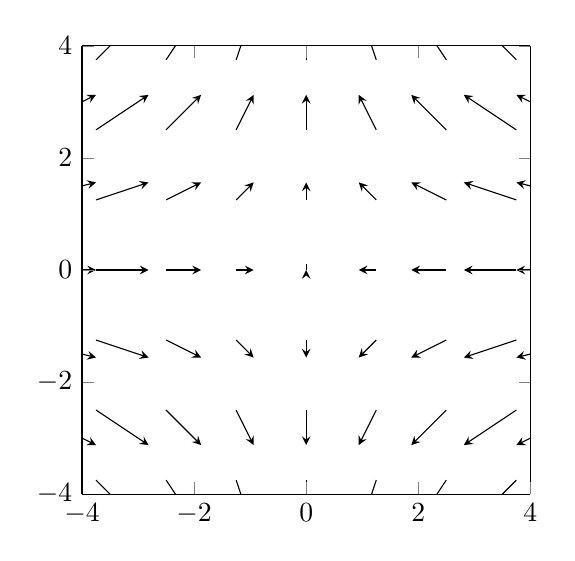
\begin{tikzpicture}
        \begin{axis}[
            xmin = -4, xmax = 4,
            ymin = -4, ymax = 4,
            zmin = 0, zmax = 1,
            axis equal image,
            view = {0}{90},
            samples = 9,
            samples y = 9,
        ]

        \addplot3[
            quiver = {
                u = {-x},
		        v = {y},
                scale arrows = 0.25,
            },
            -stealth,
        ] {0};
        \end{axis}
    \end{tikzpicture}

    \item Stable nodes:

    \begin{itemize}
        \item $B=\begin{pmatrix}
        \lambda & 0\\
        0 & \mu
        \end{pmatrix}$ with $\lambda = \mu < 0$.

        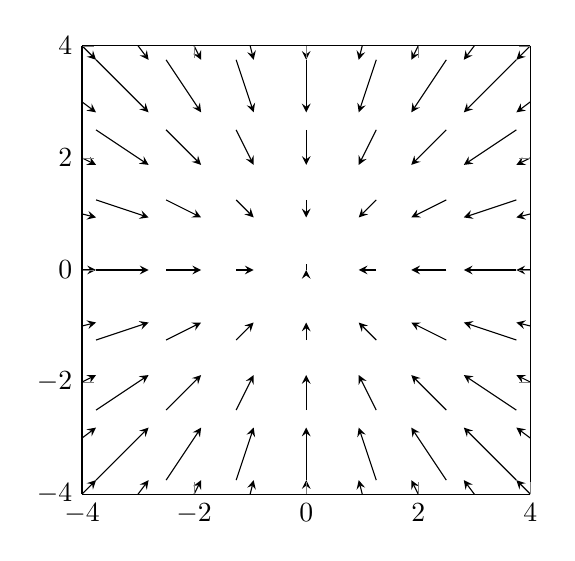
\begin{tikzpicture}
            \begin{axis}[
                xmin = -4, xmax = 4,
                ymin = -4, ymax = 4,
                zmin = 0, zmax = 1,
                axis equal image,
                view = {0}{90},
                samples = 9,
                samples y = 9,
            ]

            \addplot3[
                quiver = {
                    u = {-x},
    		        v = {-y},
                    scale arrows = 0.25,
                },
                -stealth,
            ] {0};
            \end{axis}
        \end{tikzpicture}

        \item $B=\begin{pmatrix}
        \lambda & 0\\
        0 & \mu
        \end{pmatrix}$ with $\lambda < \mu < 0$.

        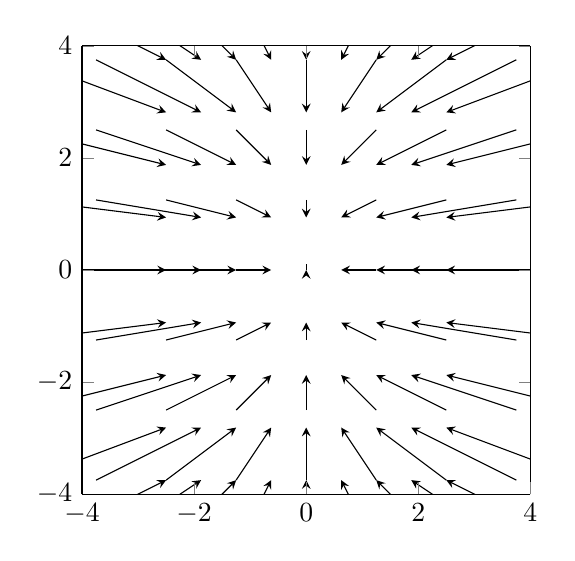
\begin{tikzpicture}
            \begin{axis}[
                xmin = -4, xmax = 4,
                ymin = -4, ymax = 4,
                zmin = 0, zmax = 1,
                axis equal image,
                view = {0}{90},
                samples = 9,
                samples y = 9,
            ]

            \addplot3[
                quiver = {
                    u = {-2*x},
    		        v = {-y},
                    scale arrows = 0.25,
                },
                -stealth,
            ] {0};
            \end{axis}
        \end{tikzpicture}

        \item $B=\begin{pmatrix}
        \lambda & 1\\
        0 & \lambda
        \end{pmatrix}$ with $\lambda < 0$.

        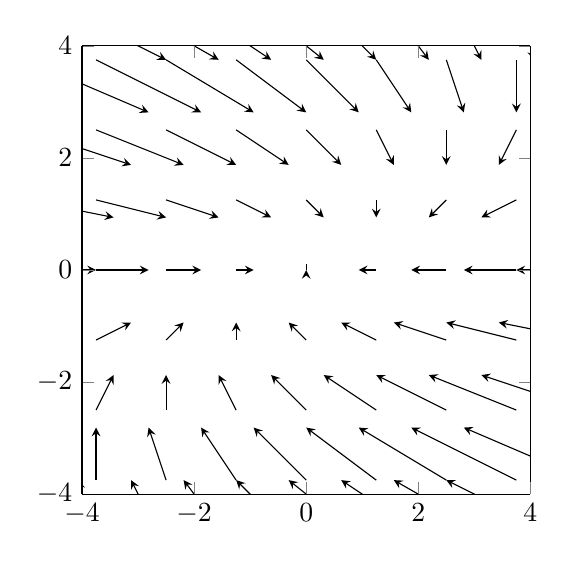
\begin{tikzpicture}
            \begin{axis}[
                xmin = -4, xmax = 4,
                ymin = -4, ymax = 4,
                zmin = 0, zmax = 1,
                axis equal image,
                view = {0}{90},
                samples = 9,
                samples y = 9,
            ]

            \addplot3[
                quiver = {
                    u = {-x+y},
    		        v = {-y},
                    scale arrows = 0.25,
                },
                -stealth,
            ] {0};
            \end{axis}
        \end{tikzpicture}
    \end{itemize}

    The flow moves towards the origin from all sides.

    \item Focus: $\begin{pmatrix}
        \mu & -\omega\\
        \omega & \mu
    \end{pmatrix}$ with $\omega \neq 0, \mu \neq 0$.

    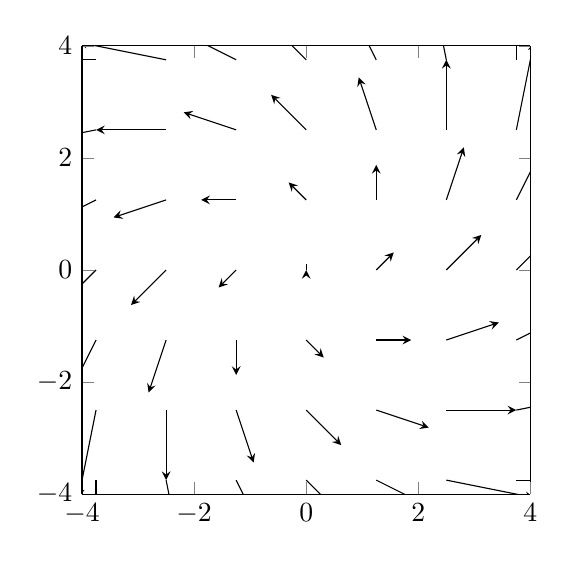
\begin{tikzpicture}
        \begin{axis}[
            xmin = -4, xmax = 4,
            ymin = -4, ymax = 4,
            zmin = 0, zmax = 1,
            axis equal image,
            view = {0}{90},
            samples = 9,
                samples y = 9,
        ]

        \addplot3[
            quiver = {
                u = {x-y},
		        v = {x+y},
                scale arrows = 0.25,
            },
            -stealth,
        ] {0};
        \end{axis}
    \end{tikzpicture}

    The flow moves around the origin and moves closer or further away from it (depending on the sign of $\mu$).

    \item Center: $\begin{pmatrix}
        \mu & -\omega\\
        \omega & \mu
    \end{pmatrix}$ with $\omega \neq 0, \mu = 0$.

    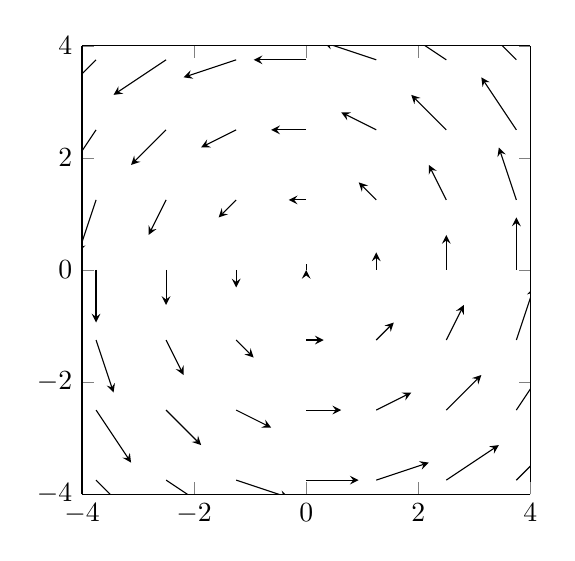
\begin{tikzpicture}
        \begin{axis}[
            xmin = -4, xmax = 4,
            ymin = -4, ymax = 4,
            zmin = 0, zmax = 1,
            axis equal image,
            view = {0}{90},
            samples = 9,
            samples y = 9,
        ]

        \addplot3[
            quiver = {
                u = {-y},
		        v = {x},
                scale arrows = 0.25,
            },
            -stealth,
        ] {0};
        \end{axis}
    \end{tikzpicture}

    The flow moves periodically around the origin in circles.
\end{enumerate}

If $0 \in \sigma(A)$ then the origin is not an isolated equilibrium.\\
%Bifurcation diagram.\\
\newline
Let $\delta = \det(A)$ and $\tau = \tr(A)$. Then the characteristic polynomial of $A$ is: $x^2-\tau x + \delta$.
Given
$$\dot x = Ax$$
we define $B := P^{-1}AP$ and $y := P^{-1}x$. Then we get
$$\dot y = P^{-1}\dot x = P^{-1}Ax = P^{-1}APy = By.$$

\subsection{Invariant subspaces}

\begin{defin}
    Let $A\in\C^{n\times n}$ and $\lambda \in \sigma(A), v \in \C^n$ is a generalized eigenvector, if
    $$(\lambda I-A)^kv=0$$
    for some $k\in\Ns$.
\end{defin}

\begin{thm}
    Let $A\in \R^{n\times n}$ with eigenvalues as follows:
    \begin{itemize}
        \item $\lambda_1,\dots,\lambda_k\in\R$

        \item $\lambda_j=\mu_j+i\omega_j, \overline{\lambda_j}=\mu_j-i\omega_j, \quad j\in\jbr{k+1,m}\quad (2m-k=n)$
    \end{itemize}

    Then the set $\{u_1,\dots,u_k,u_{k+1},v_{k+1},\dots,u_m,v_m\}$ is a basis of $\R^n$, where $u_1, \dots,u_k$ are generalized eigenvectors corresponding to $\lambda_1, \dots, \lambda_k$ and the $u_j\pm i v_j$ are generalized eigenvectors corresponding to the $\mu_j \pm i\omega_j$ where $j\in\jbr{k+1,m}$.
\end{thm}

\begin{defin}
    We define the following subspaces:
    \begin{itemize}
        \item Stable subspace: $E^s=\spanl\{u_j,\nu_j:\Re(\lambda_j)<0\}$.

        \item Center subspace: $E^c=\spanl\{u_j,\nu_j:\Re(\lambda_j)=0\}$.

        \item Unstable subspace: $E^u=\spanl\{u_j,\nu_j:\Re(\lambda_j)>0\}$.
    \end{itemize}
    We also define:
    \begin{itemize}
        \item $s(A) = \dim(E^s)$

        \item $c(A) = \dim(E^c)$

        \item $u(A) = \dim(E^u)$
    \end{itemize}
\end{defin}

\begin{exam}
    Given
    $$\begin{aligned}
    \dot x&=-2x-y\\
    \dot y &= x-2y\\
    \dot z &= 3z,
    \end{aligned}$$
    we can read the matrix
    $$A=\matthree{-2}{-1}{0}{1}{-2}{0}{0}{0}{3}.$$
    We get the following eigenpairs:
    \begin{itemize}
        \item $\lambda_1 = 3, \quad u_1 =\vecthree001$

        \item $\lambda_2 = -2+i, \quad u_2+iv_2 = \vecthree010+i\vecthree100$
    \end{itemize}
    Also
    $$\begin{array}{ll}E^s=(x,y)-\text{plane}, &\quad s(A) = 2,\\
    E^c=\{0\}, &\quad c(A)=0,\\
    E^u=z-\text{axis}, &\quad u(A)=1.
    \end{array}$$
\end{exam}

\begin{exam}
    Given
    $$\begin{array}{rcl}
    \dot x &=& -y\\
    \dot y &=& x\\
    \dot z &=& 2z,
    \end{array}$$
     we can read the matrix
    $$A=\matthree{0}{-1}{0}{1}{0}{0}{0}{0}{2}$$
    We get the following eigenpairs:
    \begin{itemize}
        \item $\lambda_1=2, \quad u_1=\vecthree001$

        \item $\lambda_2=i, \quad u_2+iv_2=\vecthree010+i\vecthree100$
    \end{itemize}
    $\begin{array}{ll}E^s=\{0\},\\E^c=(x,y)-\text{plane},\\
    E^u=z-\text{axis}.
    \end{array}$
\end{exam}

\begin{exam}
    Given
    $$\dot x=0$$
    $$\dot y = x,$$
    we can read the matrix
    $$A=\mattwo0010$$
    Since $(A-0)^2 = 0$, we get the following eigenpairs:
    \begin{itemize}
        \item $\lambda_1=0, \quad u_1=\vectwo01$

        \item $\lambda_2=0, \quad u_2\vectwo10$.
    \end{itemize}
    $\begin{array}{ll}E^s=\{0\},\\
    E^c=(x,y)-\text{plane},\\
    E^u=\{0\}.
    \end{array}$
\end{exam}

\begin{thm}
    The whole space is a direct sum of the three subspaces, meaning $\R^n=E^s\oplus E^c \oplus E^u$. Also the following statements hold:
    \begin{itemize}
        \item $E^i$ is invariant ($i = s,c,u)$.\\
        If $x(0)\in E^i$ then $x(t)=e^{At}x(0)\in E^i$ for all $t \in \R$.

        \item If $x(0) \in E^s$ then $x(t) \to 0$ as $t\to \infty$. Moreover there exist $K,\alpha > 0$, such that
        $$\|e^{At}\| \leq  Ke^{-\alpha t}$$
        for all $ t \geq 0$.

        \item If $x(0)\in E^u$ then $x(t) \to 0$ as $t \to -\infty$. Moreover there exist $L,\beta > 0$, such that
        $$\|e^{At}\|\leq Le^{\beta t}$$
        for all $t\leq 0$.\\
        %$|x(t)|\leq Le^{\beta t}|x(0)| \forall t \leq 0$
        \item $E^s = \{ p \in \R^n:e^{At}p \to 0$ as $t \to \infty\}$
        \item $E^u = \{ p \in \R^n:e^{At}p \to 0$ as $t \to -\infty\}$
    \end{itemize}
\end{thm}

\begin{defin}
    We say that a matrix $A$ is stable if $\Re(\lambda) < 0$ for all $\lambda \in\sigma(A)$.
\end{defin}

\begin{itemize}
    \item For $n=2$ the matrix $A$ is stable if and only if $\det(A) > 0$ and $\tr(A) < 0$. The characteristic polynomial is $\lambda^2-\tr(A)\lambda+\det(A)$.

    %\det(A)>M\tr(A)
    \item For $n=3$ the matrix $A$ is stable if and only if $\det(A) < 0, \tr(A)< 0,M>0$, where $M$ is the sum of the $2\times2$ principal minors
    $$M =\det\mattwo{a_{11}}{a_{12}}{a_{21}}{a_{22}} + \det\mattwo{a_{11}}{a_{13}}{a_{31}}{a_{33}}+\det\mattwo{a_{22}}{a_{23}}{a_{32}}{a_{33}}.$$
    The characteristic polynomial is (up to the faktor $(-1)$) $\lambda^3 -\tr(A)\lambda^2+M\lambda-\det(A)$.
\end{itemize}


\begin{thm}[Routh-Hurwitz]
    Each root of $x^n+b_{n-1}x^{n-1}+\dots +b_1x+b_0$ has a negative real part if and only if all the leading principal minors of $H$ are positive, where
    $$H := \begin{pmatrix}
    b_{n-1} & 1 & 0 & 0 & 0 & 0 & 0 & \dots & 0\\
    b_{n-3} & b_{n-2} & b_{n-1} & 1 & 0 & 0 & 0 & \dots & 0\\
    b_{n-5} & b_{n-4} & b_{n-3} & b_{n-2} & b_{n-1} & 1 & 0 & \dots & 0\\
    \vdots & \ddots & \ddots & \ddots & \ddots & \ddots & \ddots & \ddots & \vdots\\
    0 & \dots & 0 & 0 & b_0 & b_1 & b_2 & b_3 & b_4\\
    0 & \dots & 0 & 0 & 0 & 0 & b_0 & b_1 & b_2\\
    0 & \dots & 0 & 0 & 0 & 0 & 0 & 0 & b_0
    \end{pmatrix}.$$
\end{thm}
Applying this to $\det(xI-A)$, we get
\begin{itemize}
    \item $b_0 = (-1)^n\det(A)$

    \item $b_{n-1} = -\tr(A)$

    \item $b_j=(-1)^{n-j}\sum_{\alpha\subseteq \jbr{n}, |\alpha|=n-j} A[\alpha|\alpha]$\\
    The sum of principal minors corresponding to the rows/columns in $\alpha$.
\end{itemize}

\begin{thm}[Lyapunov]
    For $A\in \R^{n\times n}$. The following are equivalent:
    \begin{enumerate}
        \item $A$ is stable.

        \item There is a symmetric $Q>0$, such that $QA+A^TQ < 0$.

        \item For every symmetric $C <0$ there is a symmetric $Q>0$ such that $QA+A^TQ=C$.
    \end{enumerate}
\end{thm}

\begin{proof}
    We prove $(2) \Rightarrow (1) \Rightarrow (3) \Rightarrow (2)$.
    \begin{itemize}
        \item $(2) \Rightarrow (1)$: Let $Q$ be as in the statement. Now we take the time derivative of $x^TQx$. For better readability, we write $x$ instead of $x(t)$.
        $$\frac{d}{dt}(x^TQx) = \dot x^TQx+x^TQ\dot x = x^TA^TQx+x^TQAx = x^T(QA+A^TQ)x.$$
        The last expression is negative if $x(t) \neq 0$. The level sets $\{x \in \R^n: x^TQx = \gamma\}$ for $\gamma > 0$ are ellipsoids and solutions are going inwards, because if the time increases then $x^TQx$ decreases. Therefore $x(t) = e^{At}p\to 0$ as $t\to\infty$ for all $p \in \R^n$. So we get $E^s = \R^n$ and $A$ is stable.

        \item $(1)\Rightarrow (3):$ Let $C < 0$ be a symmetric matrix. Let
        $$Q = -\int_0^\infty e^{A^Tt}Ce^{At}dt.$$ It exists and is finite, because $\|e^{At}\|\leq Ke^{-\alpha t}$ for $t\geq 0$.
        \begin{itemize}
            \item Clearly $Q=Q^T>0$, because
            $$Q^T = \left(-\int_0^\infty e^{A^Tt}Ce^{At}dt\right)^T = -\int_0^\infty\left(e^{A^Tt}Ce^{At}\right)^Tdt= -\int_0^\infty\left(e^{At}\right)^TC^T\left(e^{A^Tt}\right)^Tdt = Q$$
            and
            $$x^TQx = -\int_0^\infty x^Te^{A^Tt}Ce^{At}xdt = -\int_0^\infty \left(e^{A^Tt}x\right)^TCe^{At}xdt = -\int_0^\infty y^TCydt > 0.$$

            \item We also note that
            $$QA+A^TQ = -\int_0^\infty e^{A^Tt}Ce^{At}A+A^Te^{A^Tt}Ce^{At}dt = -\int_0^\infty \frac{d}{dt}(e^{A^Tt}Ce^{At})dt =$$
            $$=-[e^{A^Tt}Ce^{At}]_{t=0}^{t=\infty} = -(0-C)=C.$$
        \end{itemize}

        \item $(3)\Rightarrow (2)$: Trivial.
    \end{itemize}
\end{proof}

\begin{defin}
    For $k \in\Ns$, we say that $h:U\to V$ is a homeomorphism (or $C^k$-diffeomorphism) if it is bijective and $h,h^{-1}$ are continuous (or $C^k$).\\
\end{defin}

\begin{defin}[Flow]
    Let  $f \in C^1(U)$. Denote the solution of
    $$\begin{aligned}\dot x(t) &= f(x(t))\\
    x(0) &= p\end{aligned}$$
    by $t \mapsto \varphi(t,p)$.\\
    The flow of $\dot x=f(x)$ is
    $$\varphi_t:\{p\in U: t\in I(p)\} \to U$$
    $$p \mapsto \varphi(t,p)$$
    For fixed $t$, the set $\varphi_t(K)$ is where a set $K$ is moved after time $t$ (as opposed to $\{\varphi(t,p)\colon t \in I(p)\}$, which is the trajectory of a single point $p$).
\end{defin}

For $\dot x = Ax$, the flow is $\varphi_t = e^{At}:\R^n\to\R^n$.

\begin{prop}
    The flow has the following properties (where these make sense):
    \begin{enumerate}
        \item $\varphi_0=id$

        \item $\varphi_s\circ\varphi_t = \varphi_{t+s}$

        \item $\varphi_t\circ\varphi_{-t}=id$
    \end{enumerate}
\end{prop}

\begin{defin}[Conjugate flow]
    We have the following ODEs
    $$\dot x=f(x)$$
    in $U$ with the flow $\varphi_t$ and
    $$\dot y=g(y)$$
    in $V$ with the flow $\psi_t$.\\
    We say that the flows $\varphi_t$ and $\psi_t$ are topologically conjugate if there is a homeomorphism $h:U\to V$ such that $h\circ \varphi_t=\psi_t\circ h$. If $h$ is a $C^k$-diffeomorphism, we say $\varphi_t$ and $\psi_t$ are $C^k$ conjugate.
\end{defin}

\begin{thm}
    If the matrices $A,B \in\R^{n\times n}$ are stable then the flows $e^{At}, e^{Bt}$ are topologically conjugate. (There is a homeomorphism $\R^n\to\R^n$ such that $h(e^{At}p)=e^{Bt}h(p)$ for all $p\in\R^n$ and $t\in\R$.)
\end{thm}

\begin{proof}[Sketch of the proof.]
    Without loss of generality, assume $B = -I$ (because being topological conjugate is an equivalence relation). Because $A$ is stable, we can find a symmetric $Q > 0$ satisfying $QA+A^TQ < 0$. Let
    $$S = \{p\in\R^n:p^TQp=1\}.$$
    Then for all $p \in \R^n\setminus \{0\}$ there is a unique $\tau(p)$ such that $e^{A\tau(p)}p\in S$. It exists, because $e^{At}p$ approaches $0$ at $\infty$ and $\infty$ at $-\infty$ and the flow is continuous. It is unique because the time derivative of $x(t)^TQx(t)$ is negative (see proof of the Lyapunov theorem). Then $\tau:\R^n \setminus\{0\} \to \R$ is continuous (because solutions depend on the initial conditions continuously).\\
    %$$e^{A\tau(e^{At}p)}\left(e^{At}p\right) = e^{A(\tau(e^{At}p)+t)}p = e^{A\tau(p)}p,$$
    Since $p$ and $e^{At}p$ are on the same orbit with a time difference of $t$, we know that
    $$\tau(e^{At}p)=\tau(p)-t.$$
    Define
    $$h(p) := \begin{cases}
        e^{(A+I)\tau(p)}p&p \neq 0\\
        0&p=0.
    \end{cases}$$
    The orbits are mapped to orbits: Indeed, for $p\neq 0$ we get
    $$h(e^{At}p)=e^{(A+I)\tau(e^{At}p)}e^{At}p = e^{(A+I)(\tau(p)-t)}e^{At}p = e^{-It}e^{(A+I)\tau(p)}p  = e^{-It}h(p).$$
    We omit the proof that $h$ is a homeomorphism.
\end{proof}

Hence, a stable focus and a stable node are topologically conjugate.

\begin{defin}
    We say that $A\in \R^{n\times n}$ is hyperbolic if $\Re(\lambda) \neq 0$ for all $\lambda \in \sigma(A)$.
\end{defin}

\begin{thm}
    For $A, B \in \R^{n\times n}$ hyperbolic matrices, the following statements are equivalent:
    \begin{itemize}
        \item $s(A) = s(B)$ and $u(A) = u(B)$

        \item $e^{At}$ and $e^{Bt}$ are topologically conjugate.
    \end{itemize}
\end{thm}

\begin{exam}
    The matrices
    $$A = \mattwo{0}{-2}{2}{0}, \quad B=\mattwo{0}{-1}{1}{0}$$
    are not topologically conjugate. To show this, we compute
    $$e^{At} = \mattwo{\cos(2t)}{-\sin(2t)}{\sin(2t)}{\cos(2t)}, \quad e^{Bt} = \mattwo{\cos(t)}{-\sin(t)}{\sin(t)}{\cos(t)}.$$
    Suppose that there is a homeomorphism $h$ such that
    $$h(e^{At}p) = e^{Bt}h(p)$$
    for all $p\in\R^2$ and for all $t\in \R$. Setting $t = \pi$ yields $h(p)= -h(p)$ and then $h(p) = 0$ for all $p \in \R^2$, which is a contradiction.
\end{exam}

\begin{thm}
    If $c(A) = c(B) =n$ then $e^{At}$ and $e^{Bt}$ are topologically conjugate if and only if $A$ and $B$ are similar matrices.
\end{thm}

\begin{thm}
    The flows $e^{At}, e^{Bt}$ are topologically conjugate if and only if $s(A) = s(B), u(A) = u(B), c(A) = c(B)$ and $A|_{E^c(A)}, B|_{E^c(B)}$ are similar.
\end{thm}

\begin{prop}
    $A$ and $B$ are $C^1$-conjugate if and only if $A$ and $B$ are similar.
\end{prop}

\begin{proof}
    We need to show both directions.
    \begin{itemize}
        \item $\Leftarrow$: We just use the transformation matrix as a homeomorphism.

        \item $\Rightarrow$: By definition $h(e^{At}p)=e^{Bt}h(p)$ for all $t,p$. Differentiate with respect to $p$ and set $p = 0$.
        $$h'(e^{At}0)e^{At}=e^{Bt}h'(0)$$
        $$h'(0)e^{At}=e^{Bt}h'(0),$$
        where $h'$ is the Jacobian matrix of $h$. Differentiate with respect to $t$ and set $t=0$.
        $$h'(0)Ae^{A0}=Be^{B0}h'(0)$$
        Let $P := (h'(0))^{-1}$. Then
        $$B=P^{-1}AP.$$
    \end{itemize}
\end{proof}

Hence $C^1$-conjugacy is too strong: e.g.

$$\dot x = -x$$
and
$$\dot y = -2y$$
are not $C^1$-conjugate.

\begin{rem}[Related to Routh-Hurwitz]
    Given the real polynomial $x^n+b_{n-1}x^{n-1} +\dots + b_0$, where all roots have negative real parts. Then $b_{n-1} > 0, \dots, b_0 > 0$.
\end{rem}

\begin{proof}
    We first consider the simplest cases.
    \begin{itemize}
        \item $n=1$: The polynomial $x + b_0$ has the root $-b_0$. By assumtion, it has to have a negative real part, so $b_0 > 0$.

        \item $n=2$: The polynomial $x^2+b_1x+b_0=(x-\lambda_1)(x-\lambda_2)$ has the roots $\lambda_1$ and $\lambda_2$, which have a negative real part. Then $b_0 = \lambda_1\lambda_2$ and $b_1 = -\lambda_1-\lambda_2$. Obviously $b_1 > 0$. If $\lambda_1$ and $\lambda_2$ are real, then they are negative and $b_0>0$. Otherwise, they are of the form $\mu\pm i\omega$. In this case, $b_0 = (\mu+i\omega)(\mu-i\omega) = \mu^2+\omega^2 > 0$.

        \item For higher degree, find the decomposition of the polynomial to irreducible factors, which leads to linear and quadratic polynomials. Then each coefficient of the factors is positive. Multiplying those factors together, we get positive coefficients of the whole polynomial.
    \end{itemize}
\end{proof}

\subsection{Stability of equilibria}

Let the following general differential equation be given:
$$\dot x(t)=f(x(t)),$$
where $f \in C^1(U)$. For $p\in U$ and $ t\mapsto \phi(t,p)$ denote the solution for which $x(0)=p$ holds (on a maximal time interval $I(p)$).

\begin{defin}
    We say that $p\in U$ is an equilibrium if $f(p) = 0$. In this case, $\phi(t,p)$ is constant over time. So $\phi_t(p)=p$, meaning that $p$ is a fixed point of the flow for all $t \in \R$.
\end{defin}

\begin{defin}
    An equilibrium $p$ is Lyapunov stable if for all $\epsilon > 0$ there is a $\delta > 0$ such that $|q-p| < \delta$ implies $|\phi(t,q)-p| < \epsilon$ for all $t\geq 0$. Otherwise $p$ is called unstable.
\end{defin}

\begin{defin}
    An equilibrium is called attracting if there is a neighborhood $U_0 \subseteq U$ of $p$ such that $\lim_{t\to\infty} \phi(t,q)=p$ for all $q\in U_0$.
\end{defin}

\begin{defin}
    An equilibrium is said to be asymptotically stable if it is Lyapunov stable and attracting.
\end{defin}

\begin{exam}[An attracting equilibrium that is not Lyapunov stable]
    Let the following system be given in polar coordinates
    $$\begin{array}{ll}\dot r=r(1-r), &\quad r\geq 0,\\
    \dot \theta=\sin^2\left(\half\theta\right), &\quad (0\leq \theta < 2\pi).\end{array}$$

    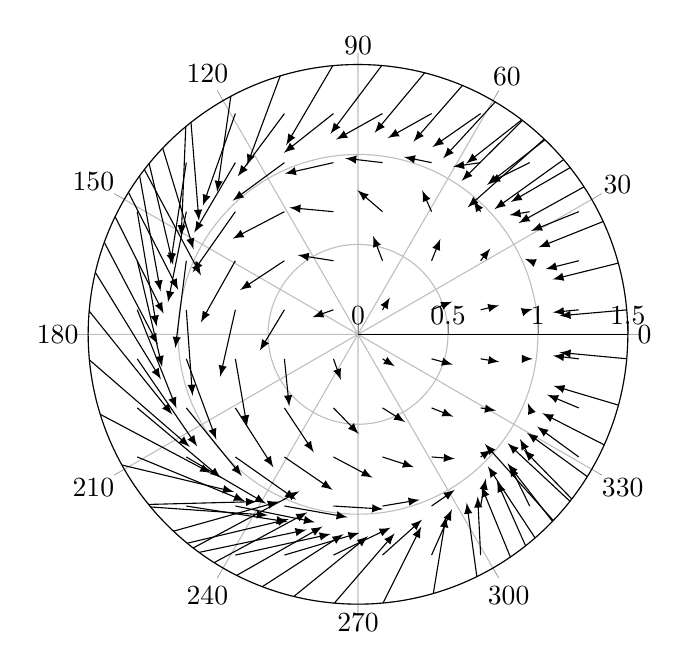
\begin{tikzpicture}
            \begin{polaraxis}[
                ymax = 1.5,
            ]

            \addplot3[
                samples=12,
                samples y=12,
                quiver = {
                    u = {deg(sin(atan2(y,x)/2)^2)},%{veclen(y,x)*(1-veclen(y,x))},
    		        v = {veclen(y,x)*(1-veclen(y,x))},%{sin(atan2(y,x)/2)^2},
                    scale arrows = 0.5,
                },
                -latex,
                domain=-1.5:1.5,
                domain y=-1.5:1.5,
                data cs=cart
            ] (x, y, 0);
            \end{polaraxis}
        \end{tikzpicture}

    The point $(r^*,\theta^*) = (1,0)$ is not Lyaponov stable, but attracts $\R^2\setminus \{0\}$. In the polar form it attracts all points with $r > 0$ and $0\leq \theta < 2\pi$.
\end{exam}

\begin{exam}
    Given
    $$\begin{array}{rcl}\dot x &=& -y-x^3\\
    \dot y &=& x-y^3.\end{array}$$
    Let $V(x,y):= x^2+y^2, \R^2\to\R$. Taking the derivative with respect to $t$ gives us
    $$\frac{d}{dt}V(x,y) = \nabla V(x,y)\cdot\vectwo{\dot x}{\dot y} = 2(x\dot x+y\dot y) =  2(x(-y-x^3)+ y(x-y^3)) = -2(x^4+y^4) < 0.$$
\end{exam}

In general, $V \in C^1(\Rn,\R)$. When differentiating with respect to $t$ and setting $t=0$ we get
$$\frac{d}{dt} V(x)|_{t=0} = \nabla V(x)\cdot \dot x|_{t=0} = \nabla V(x)\cdot f(x)|_{t=0}.$$
So
$$\dot V(x) := \nabla Vf(x) := \nabla V(x)\cdot f(x), \dot V: U\to \R$$
is the derivative of $V$ with respect to $f$.

\begin{defin}
    Let $p$ be an equilibrium and $U_0 \subseteq U$ an open neighbourhood of $p$. A function $V: U_0\to \R$ is called a Lyapunov function for $p$ if:
    \begin{enumerate}
        \item $V(p) = 0$ and $V(x) > 0$ for $x \in U_0\setminus\{p\}$.

        \item $V$ is continuous in $U_0$, $C^1$ in $U_0\setminus \{p\}$ and $\dot V(x)\leq 0$ for $x \in U_0\setminus \{p\}$.
    \end{enumerate}
    If $\dot V(x) < 0$ for all $x\in U_0\setminus\{p\}$, then we call it a strict Lyapunov function for $p$.
\end{defin}

We can imagine that each orbit moves along $V$ such that the value of $V$ doesn't increase. So as long as the orbit starts close at $p$, it stays close to it.

\begin{hw}
    Consider
    $$\dot x = f(x)$$
    in $\R$ with an equilibrium $f(p)=0$. Show that $p$ is asymptotically stable if and only if $V(x) = |x-p|$ is a strict Lyapunov function for $p$ in a neighborhood.
\end{hw}

\begin{hw}
    Pendulum with friction: Given
    $$\begin{aligned}\dot x&=y\\
    \dot y &= \sin x-\delta y\end{aligned}$$
    where $\delta \geq 0$. Show that
    $$V(x,y) := \half{y^2}-\cos x$$
    is a Lyapunov function at the origin.
\end{hw}

\begin{hw}
    For which $A\in\R^{n\times n}$ is the origin of $\dot x = Ax$ Lyapunov stable?
\end{hw}

\begin{thm}[Lyapunov, 1892]
    The following statements hold:
    \begin{enumerate}
        \item If there is a Lyapunov function for the equilibrium $p$ then $p$ is Lyapunov stable.

        \item If there is a strict Lyaponov function for the equilibrium $p$ then $p$ is asymptotically stable.
    \end{enumerate}
\end{thm}

\begin{proof}
    For the proof, we use some $\epsilon$-$\delta$-tricks.
    \begin{enumerate}
        \item Let $\epsilon > 0$ such that
        $$\overline{B_\epsilon(p)} \subseteq U_0.$$
        Let
        $$\alpha := \min_{|x-p|=\epsilon}V(x) > 0.$$
        Clearly, $V(p)<\alpha$. Let $\delta > 0$ such that $|x-p|<\delta$ implies $V(x) < \alpha$ (recall $V$ is continuous).\\
        Then for $q$ with $|q-p| < \delta$ we have $V(\varphi(t,q))< \alpha$ for $t \geq 0$. This is, because $V(\varphi(0,q)) = V(q) < \alpha$ and $\dot V \leq 0$. So the flow will never intersect the sphere $\{x\in\Rn:|x-p| = \epsilon\}$. Therefore we get $|\varphi(t,q)-p|<\epsilon$ for $t\geq 0$.

        \item We show that $\lim_{t\to\infty}\varphi(t,q) = p$ if $|q-p|<\delta$. Since $t\mapsto V(\varphi(t,q))$ is monotone decreasing, the following limit exists:
        $$\lim_{t\to\infty}V(\varphi(t,q))=:c \geq 0.$$
        \begin{itemize}
            \item If $c = 0$, then the orbit stays in a compact neighborhood of $p$, since $V$ is Lyapunov stable. Therefore the orbit accumulates at a certain point $r$. Since $c = 0$, the only accumulation point possible is $p$. So $\lim_{t\to\infty} \varphi(t,q) = p$.

            \item If $c > 0$ then there is a $\gamma > 0$ such that $|\varphi(t,q)-p|\geq \gamma$ for $t\geq 0$. On the compact set
            $$\{x\in U_0: \gamma \leq |x-p|\leq \epsilon\},$$
            we get that
            $$\dot V(x)\leq -\beta < 0$$
            for every $x$. Therefore $V(\varphi(t,q))\to-\infty$ as $t\to\infty$, which is a contradiction.
        \end{itemize}
    \end{enumerate}
\end{proof}

\begin{hw}
    Given the following scalar ODE:
    $$\dot x = x^3 \sin^2\left(\reci x\right)$$
    Is the origin Lyapunov stable? Can you find a Lyapunov function?
\end{hw}

\begin{hw}
    Prove the following statements about the pendulum with friction:
    \begin{itemize}
        \item If $\delta = 0$ then the origin is Lyapunov stable.

        \item If $\delta > 0$ then the origin is asymptotically stable.
    \end{itemize}
\end{hw}

\begin{hw}
    Is the following statement true or false? Give a proof or a counterexample.
    \begin{itemize}
        \item If $V:\R^n\to\R$ is a strict Lyapunov function for the equilibrium $p$, then $\lim_{t\to\infty} \varphi(t,q) = p$ for all $q \in\R^n$.\\
    \end{itemize}
\end{hw}

\begin{hw}
    Lorenz:\\
    Given the following system of equations:
    $$\begin{array}{rcl}\dot x&=&\sigma(y-x)\\
    \dot y &=& \rho x-y-xz\\
    z &=& xy-\beta z\end{array}$$
    Show that the origin is globally asymptotically stable if $0<\rho < 1$.\\
    Hint: $V(x,y,z) = \rho x^2+\sigma y^2+\sigma z^2$
\end{hw}

Given
$$\dot x(t)=f(x(t))$$
where $f \in C^1(U)$ and $f(p) = 0$. Then
$$f(x)=f'(p)(x-p)+r(x)$$
where $f'$ is the Jacobin matrix of $f$.
$$f'=\matthree{\partial_1f_1}{\dots}{\partial_nf_1}{\vdots}{}{\vdots}{\partial_1f_n}{\dots}{\partial_nf_n}=(\partial_jf_i)_{i,j=1}^n$$
Also $r(p) = 0$ and $\lim_{x\to\infty}\frac{r(x)}{|x-p|}=0$. Let $A := f'(p)$.
\begin{thm}
    If $A$ is stable then $p$ is asymptotically stable for $\dot x=f(x)$.
\end{thm}

\begin{proof}
    Assume without loss of generality that $p=0$. Let $Q = Q^T > 0$ such that $QA+A^TQ<0$.\\
    We claim that $V(x)=x^TQx$ is a strict Lyapunov function for $p$. So we need to show that $\dot V(x) < 0$ for $x \neq p$.\\
    $$\dot V(x) = \nabla V(x)\cdot f(x)=2x^TQ (Ax+r(x))$$
    Because $x^TQAx$ is a scalar, we can transpose it, to get to $x^TA^TQx$. Then we get
    $$\dot V(x) = x^T(QA+A^TQ)x + 2x^T Q r(x).$$
    We define the inner product
    $$\jbr{x,y}:=x^TQy$$
    with the induced norm
    $$\|x\|^2 := \jbr{x,x}=x^TQx.$$
    Now let's calculate the following quotient:
    $$\frac{\dot V(x)}{V(x)}=\frac{x^T(QA+A^TQ)x}{x^TQx}+2\frac{\jbr{x,r(x)}}{\|x\|^2}$$
    The first term is smaller than or equal $-c$ for $c := \min_{\|x\|=1}\left(\frac{-x^T(QA+A^TQ)x}{x^TQx}\right)>0$. For the second term:
    $$\frac{\jbr{x,r(x)}}{\|x\|^2}\leq \frac{\|x\|\|r(x)\|}{\|x\|^2} = \frac{\|r(x)\|}{\|x\|} \to 0$$
    as $x \to 0$. Therefore, $\frac{\dot{V}}{V}$ is negative in a neighborhood of the origin. So for $x \neq 0$ close to $p$, $\dot V(x) < 0$ so $V$ is a Lyapunov function.
\end{proof}

\begin{hw}
    Show that the origin is asymptotically stable for the pendulum with friction $(\delta > 0)$ (linearize).
\end{hw}

\begin{defin}
    An equilibrium $p$ is hyperbolic if $f'(p) \in \R^{n\times n}$ has no eigenvalue with zero real part.
\end{defin}

\begin{thm}[Hartman-Grobman]
    If $f$ is $C^1$ and $p$ is a hyperbolic equilibrium then the local flow $\varphi_t$ is topologically conjugate to the local flow of
    $$\dot y = f'(p)y$$
    at the origin. (There is an open neighborhood $U_0$ of $p$, an open neighborhood $U_1$ of $0 \in \R^n$ and a homeomorphism $h:U_0 \to U_1$ such that
    $$h\circ \varphi_t = e^{At}\circ h$$
    (here $A := f'(p)$) where this is defined ($\varphi_t(x) \in U_0$).)\\
    (Simon, Perko, Teschl)
\end{thm}

\begin{defin}
    Let $p$ be an equilibrium and $A = f'(p)$.

    \begin{itemize}
        \item We say that $p$ is a sink if $\Re(\lambda) < 0$ for all $\lambda \in \sigma(A)$.

        \item We say that $p$ is a source if $\Re(\lambda)>0$ for all $\lambda \in \sigma(A)$.

        \item We say that $p$ is a saddle if it is hyperbolic, meaning th there is a $\lambda_1 \in \sigma(A)$ with $\Re(\lambda_1)<0$ and $\lambda_2 \in \sigma(A)$ with $\Re(\lambda_2)> 0$.
    \end{itemize}
\end{defin}

\begin{hw}
    Classify all of the equilibria of
    $$\begin{aligned}\dot x&=x^2-y^2-1\\
    \dot y &= 2y.\end{aligned}$$
\end{hw}

\begin{exam}
    Show that the flows of
    $$\begin{aligned}\dot x &= -x\\
    \dot y &= y+x^2\end{aligned}$$
    and
    $$\begin{aligned}\dot u &= -u\\
    \dot v &= v\end{aligned}$$
    are topologically conjugate (not only locally, but even globally).\\
    Let
    $$h:(x,y)\mapsto (x,y+\frac{x^2}{3}).$$
    Then
    $$h^{-1}: (u,v)\mapsto (u,v-\frac{u^2}{3})$$ and $h$ is a homeomorphism. Let
    $$(u,v) = h(x,y)$$
    or
    $$\begin{aligned}u&=x\\
    v&=y+\frac{x^2}{3}\end{aligned}.$$
    Then
    $$\begin{aligned}\dot u &= \dot x=-x = -u\\
    \dot v &= \dot y + \frac{2}{3}x\dot x=y+x^2+\frac{2}{3}(-x^2)= y+\frac{x^2}{3}=v.\end{aligned}$$
\end{exam}

\subsection{Polar coordinates}

If there is a system in Cartesian form like
$$\begin{aligned}\dot x &= f(x,y)\\
\dot y &= g(x,y)\end{aligned}$$
we can get to a system in polar form like
$$\begin{aligned}\dot r = F(r,\theta)\\
\dot \theta = G(r,\theta)\end{aligned}$$
where
$$\begin{aligned}&x = r\cos(\theta), &y = r\sin(\theta)\\
&r = \sqrt{x^2+y^2}, &\theta = \arctan(y/x).\end{aligned}$$
Using some derivative tricks, we get
$$\dot x = \dot r \cos(\theta) +r(-\sin(\theta))\dot \theta, \quad \dot y = \dot r \sin(\theta) + r \cos(\theta) \dot \theta,$$
$$\dot r = \frac{2x\dot x +2y \dot y}{2\sqrt{x^2+y^2}}, \quad \dot \theta = \frac{\frac{\dot yx - y\dot x}{x^2}}{1+\frac{y^2}{x^2}} = \frac{\dot yx-y\dot x}{x^2+y^2},$$

$$\dot x=-y\dot \theta +x\frac{\dot r}{r}, \quad
\dot y = x\dot \theta +y\frac{\dot r}{r},$$
$$\dot r = \frac{x\dot x + y\dot y}{r}, \quad
\dot \theta = \frac{x\dot y-\dot xy}{r^2}.$$

Linearization at a nonhyperbolic equilibrium (these are situations, where the Hartman-Grobman theorem does not apply):

\begin{exam}
    1D
    \begin{itemize}
        \item Given
        $$\dot x = -x^3,$$
        the equilibrium $0$ attracts from both sides.

        \item Given
        $$\dot x = x^3,$$
        the equilibrium $0$ repells.

        \item Given
        $$\dot x = x^2,$$
        the flow goes to the right.

        \item Given
        $$\dot x = 0,$$
        everything is stationary. (This is the linearization of all three equations above.)
    \end{itemize}

\end{exam}

\begin{exam}
    2D
    \begin{itemize}
        \item Given
        $$\begin{aligned}\dot r &= -r^3\\
        \dot \theta &= 1\end{aligned}$$
        in polar coordinates or
        $$\begin{aligned}\dot x &= -y-xy^2-x^3\\
        \dot y &= x-y^3-x^2y\end{aligned}$$
        in Cartesian coordinates, the flow spirals inwards. So the origin is asymptotically stable.

        \item Given
        $$\begin{aligned}\dot r &= r^3\\
        \dot \theta &= 1\end{aligned}$$
        in polar coordinates or
        $$\begin{aligned}\dot x &= -y+xy^2-x^3\\
        \dot y &= x+y^3+x^2y\end{aligned}$$
        in Cartesian coordinates, the flow spirals outwards. So the origin is repelling.

        \item Given
        $$\begin{aligned}\dot r &= 0\\
        \dot \theta &= 1+r\cos(\theta)\end{aligned}$$
        in polar coordinates or
        $$\begin{aligned}\dot x &= -y-xy\\
        \dot y &= x+x^2\end{aligned}$$
        in Cartesian coordinates, we get a center at the origin.

        \item All three examples above have the same linearization:
        $$\begin{aligned}\dot x &= -y\\
        \dot y &= x\end{aligned}.$$
        Here the flow moves in circles around the origin.
    \end{itemize}
\end{exam}

\subsection{Asymptotic behavior}

What do solutions do as $t \to \infty$? Given
$$\dot x(t) = f(x(t))$$
where $f \in C^1(U, \Rn)$ and $t \mapsto \varphi(t,p)$ is the solution with $x(0) = p$.

\begin{defin}
    For $p \in U$, the $\omega$-limit of $p$ is
    $$\omega(p)=\{q\in U: \exists (t_n)_{n\in\N} \subseteq \R \text{ such that } \lim_{n\to\infty}t_n = \infty \text{ and } \lim_{n\to\infty}\varphi(t_n,p)=q\}.$$
    For $p\in U$, the $\alpha$-limit of $p$ is
    $$\alpha(p) = \{q\in U:\exists (t_n)_{n\in\N} \subseteq \R \text{ such that }\lim_{n\to\infty}t_n=-\infty \text{ and } \lim_{n\to\infty}\varphi(t_n,p)=q\}.$$
\end{defin}

\begin{exam}
Let's do some examples.
\begin{enumerate}
    \item Given:
    $$\begin{aligned}\dot x&=x\\
    \dot y &= -y.\end{aligned}$$
    \begin{itemize}
        \item If $p = 0$ then $\alpha(p) = \{0\}$ and $\omega(p)=\{0\}.$

        \item If $p \neq 0$ is on the $x$-axis then $\alpha(p)=\{0\}$ and $\omega(p)=\emptyset$.

        \item If $p \neq 0$ is on the $y$-axis then $\alpha(p) = \emptyset$ and $\omega(p) = \{0\}$.

        \item If $p$ is on no axis then $\alpha(p) = \emptyset$ and $\omega(p) = \emptyset$.
    \end{itemize}

    \item Given:
    $$\begin{aligned}\dot x &= -y+x(1-x^2-y^2)\\
    \dot y &= x+y(1-x^2-y^2)\end{aligned}$$
    or
    $$\begin{aligned}\dot r &= r(1-r^2)\\
    \dot \theta &= 1\end{aligned}$$

    \begin{itemize}
        \item If $p = 0$ then $\alpha(p) = \{0\}$ and $\omega(p) = \{0\}$.

        \item If $p \neq 0$ is inside the unit circle then $\alpha(p) = \{0\}$ and $\omega(p)$ is the boundary of the unit circle.

        \item If $|p| = 1$ then $\alpha(p)$ and $\omega(p)$ are the boundary of the unit circle.

        \item If $p$ is outside the unit circle then $\alpha(p)=\emptyset$ and $\omega(p)$ is the boundary of the unit circle.
    \end{itemize}



    \item Given:
    $$\begin{aligned}\dot x &= -y+x(1-x^2-y^2)\\
    \dot y &= x+y(1-x^2-y^2)\\
    \dot z &= \beta > 0 \text{ (constant)} \end{aligned}$$
    Then for every $p \in \R^3$ we get $\alpha(p) = \omega(p) = \emptyset$.

    \item Same as 3, but identify $0$ and $2\pi$ on the $z$-axis. Then the invariant cylinder becomes an invariant torus. If $\beta\in\Q$ then the torus is filled with periodic orbits (and the $\omega$-limit is one of these periodic orbits, provided $p$ is not on the $z$-axis).\\
    If $\beta \notin \Q$ then there are everywhere dense orbits on the torus and $\omega(p)$ is the torus for all $p$ not on the $z$-axis.

    \item Lorenz equation: Strange attractor.
\end{enumerate}
\end{exam}

\begin{thm}
    The following statements are true:
    \begin{enumerate}
        \item $\omega(p)$ is closed.

        \item $\omega(p)$ is invariant (if $q \in \omega(p)$ then $\varphi(t,q) \in \omega(p)$ for all $t \in \mathbb{R}$).

        \item If $\{\varphi(t,p):t\geq 0\}$ is bounded then $\omega(p)$ is nonempty an connected.
    \end{enumerate}
\end{thm}

\begin{proof}
    Let's go through the proof.
    \begin{enumerate}
        \item Let $q\notin \omega(p)$. Then there is an open neighborhood $U_0\subseteq U$ of $q$ and $T > 0$, such that $\varphi(t,p)\notin U_0$ for all $t \geq T$. So after time $T$, the solution does not enter $U_0$. Therefore $U_0 \subseteq \omega(p)^c$ implying that $\omega(p)^c$ is open and $\omega(p)$ is closed.

        \item Fix $q \in \omega(p)$. Then there is a sequence $(t_n)_{n\in\N} \subseteq \R$, such that $\lim_{n\to\infty}t_n = \infty$ and $\lim_{n\to \infty}\varphi(t_n,p) = q$.\\
        Fix $t\in\R$ and let $\tau_n = t_n+t$. Then $\lim_{n\to\infty}\tau_n=\infty$ and $$\lim_{n\to\infty}\varphi(\tau_n,p) = \lim_{n\to\infty}\varphi(t_n+t,p) = \lim_{n\to\infty}\varphi(t,\varphi(t_n,p))=\varphi(t,q)$$
        (because of the continuous dependence of solutions on the initial conditions). Therefore, we get $\varphi(t,q) \in \omega(p)$.

        \item The solution lies in a compact set $K$. Take any sequence $(t_n)_{n\in\N}\subseteq\R$ such that $\lim_{n\to\infty}t_n=\infty$. Then $(\varphi(t_n,p))_{n\in\N} \subseteq K$ and there is a subsequence $(\varphi(t_{n_k},p))_k$ such that $\lim_{k\to\infty}\varphi(t_{n_k},p) \in K$ exists. Therefore $\omega(p) \neq \emptyset$.\\
        Now we show that $\omega(p)$ is connected. By way of contradiction, assume there exist $G_1, G_2$ open sets such that:
        \begin{itemize}
            \item $G_1$ and $G_2$ are disjoint.

            \item $G_1 \cup G_2 \supseteq \omega(p)$.

            \item $G_1 \cap \omega(p) \neq \emptyset$ and $G_2 \cap \omega(p) \neq \emptyset$.
        \end{itemize}

        Then there are sequences $(t_n)_{n\in\N}, (\tau_n)_{n\in\N} \subseteq \R$ such that
        $\lim_{n\to\infty} t_n=\infty$, $\lim_{n\to\infty}\tau_n=\infty$,
        $$\lim_{n\to\infty}\varphi(t_n,p)=q_1 \in G_1 \cap \omega(p)$$
        and
        $$\lim_{n\to\infty}\varphi(\tau_n,p)=q_2  \in G_2 \cap \omega(p),$$
        where $t_1 < \tau_1 < t_2 < \tau_2 < \dots$.\\
        Let $\theta_n$ be in the interval $(t_n,\tau_n)$ such that $\varphi(\theta_n,p)\notin G_1 \cup G_2$. Then as above $(\varphi(\theta_n,p))_{n\in\N}$ has a convergent subsequence, thus we found a point in $\omega(p) \setminus(G_1 \cup G_2)$ which is a contradiction.
    \end{enumerate}
\end{proof}

\begin{hw}
    Sketch a 2D example with nonempty and disconnected $\omega$-limit set.
\end{hw}

In a one-dimensional system the $\omega$-limit of a point $p$ is either $\emptyset$ or $\{q\}$, where $q$ is an equilibrium. What happens in the two-dimensional case?

\begin{thm}[Poincar\'e-Bendixson]
    Let $U \subseteq \R^2$ be open. Let
    $$\dot x(t)=f(x(t))$$
    be given where $f\in C^1(U,\R^2)$. Let $K \subseteq U$ be a forward invariant ($p \in K$ implies $\varphi(t,p)\in K$ for all $t \geq 0$), compact set with finitely many equilibria. Then for any $p \in K$ the set $\omega(p)$ is one of the following:
    \begin{itemize}
        \item $\omega(p) = \{q\}$, where $q$ is an equilibrium.

        \item $\omega(p) = \gamma$, where $\gamma$ is a closed orbit (the image of a periodic solution).

        \item $\omega(p)$ is the union of $\{q_1, \dots ,q_n\}$ and countably many non closed orbits $\gamma$ such that $\alpha(\gamma) = q_i$ and $\omega(\gamma)=q_j$.
    \end{itemize}
\end{thm}

\begin{defin}
    If $q$ is an equilibrium and $\gamma$ is an orbit with $\lim_{t \to \pm\infty}\gamma(t) = q$, then $\gamma$ is called a homoclinic orbit.
\end{defin}

\begin{defin}
    If $q_1, q_2$ are two different equilibria and $\gamma$ is an orbit with $\lim_{t\to-\infty}\gamma(t) = q_1$ and $\lim_{t\to\infty}\gamma(t) = q_2$, then $\gamma$ is called a heteroclinic orbit.
\end{defin}

\begin{exam}
    The system
    $$\begin{aligned}\dot x &= x(1-x)(x-y)\\
    \dot y &= y(1-y)(2x-1)\end{aligned}$$
    has an attractin rectangle.
\end{exam}

\begin{rem}
    The Poincar\'e-Bendixson-Theorem does not apply to 2D manifolds other than subsets of $\R^2$ or the $2$-sphere.
\end{rem}

For instance, let
$$\dot x = v$$
for $v \in \R^2$ such that $\frac{v_1}{v_2}\notin \Q$ in the $2$-torus $\mathbb{T}^2$.
$$x(t)=tv+p$$
is dense in $\mathbb{T}^2$ and $\omega(p) = \mathbb{T}^2$.

\begin{defin}
    Given
    $$\begin{aligned}
        \dot x_1 = f_1(x)\\
        \dot x_2 = f_2(x)\\
        \vdots\\
        \dot x_n = f_n(x)
    \end{aligned}$$
    for $f = (f_1, \dots, f_n) \in C(U)$. For $i \in \jbr{n}$, we define $\{x \in U: f_i(x) = 0\}$ the $x_i$-nullcline.
\end{defin}

\paragraph{Chlorine dioxide-Iodine-Malonic-Acid reaction: $(X = I, Y = ClO_2^-)$}
Given
$$\begin{aligned} \dot x &= a-x-\frac{4xy}{x^2+1}\\
\dot y &= bx\left(1-\frac{y}{x^2+1}\right),\end{aligned}$$
where $a,b > 0$ and $x,y\geq 0$. We first compute the nullclines.
$$\begin{aligned}\dot x = 0 &\Leftrightarrow y = \frac{(a-x)(x^2+1)}{4x}\\
\dot y = 0 &\Leftrightarrow y = x^2+1\end{aligned}$$
Solving this system of equation gives
$$x^* = \frac a5,\quad y^* = 1+(x^*)^2.$$
Now we compute the Jacobian matrix $J$ at $(x^*,y^*)$.
$$J (x^*,y^*) = \reci{(x^*)^2+1}\mattwo{3(x^*)^2-5}{-4x^*}{2b(x^*)^2}{-bx^*}$$
To get information about the eigenvalues, we calculate the determinant and the trace of it.
$$\det J(x^*,y^*)=\frac{5bx^*}{(x^*)^2+1}>0$$
$$\tr J(x^*,y^*)=\frac{3(x^*)^2-bx^*-5}{(x^*)^2+1}$$
$$\sgn(\tr J(x^*,y^*)) = \sgn(3a^2-5ab-125)$$
\begin{itemize}
    \item For $b > \frac35a-\frac{25}a$ it is asymptotically stable.

    \item For $b < \frac35a-\frac{25}a$ it is repelling, and, by the Poincar\'e-Bendixson Theorem, there is a closed orbit.

    \item At $b = \frac35a-\frac{25}a$ a supercritical Andronov--Hopf bifurcation occurs (such a bifurcation will be discussed on May 8th).
\end{itemize}

\begin{defin}
    A limit cycle is a closed orbit $\gamma$ which is the $\omega$-limit or $\alpha$-limit of at least one point outside $\gamma$.
\end{defin}

\begin{defin}
    A periodic attractor is a closed orbit such that for all $p$ in a neighborhood of $\gamma$, we get
    $$\omega(p)=\gamma.$$
    (Note: a neighborhood of $\gamma$ in $\R^2$ is an annulus, in $\R^n$ it is a torus.)
\end{defin}

\begin{hw}
    Given
    $$\begin{aligned}
        \dot x &= y+xh(r)\\
        \dot y &= x+yh(r)\\
        r &= \sqrt{x^2+y^2},
    \end{aligned}$$
    write in polar coordinates and find $h$ such that there are infinitely many limit cycles.
\end{hw}

\begin{thm}[Green's theorem]
    Let $F:\R^2\to\R^2$ be smooth, $D\subseteq \R^2$ be a simply connected region, $\gamma$ be its boundary and
    $n: \gamma \to\R^2$ is the outward facing unit normal vector field. Then
    $$\int_\gamma F\cdot n=\iint_D\divg F.$$
    With $F=(P,Q)$ this reads as
    $$\oint_\gamma Pdy-Qdx = \iint_D\partial_x P+\partial_y Q.$$

\end{thm}

\begin{thm}[Bendixson-Dulac criterion]
    Given
    $$\begin{aligned}
        \dot x = f(x,y)\\
        \dot y = g(x,y)
    \end{aligned}$$
    where $(f,g):D \to\R^2$ is $C^1$ and $D \subseteq \R^2$ is a simply connected region.\\
    If there is an $h:\R^2\to\R$ which is $C^1$ such that $\text{div}(hf,hg) > 0$ in $D$ (or $\text{div}(hf,hg)<0$ in $D$) then there is no closed orbit that lies entirely in $D$.
\end{thm}

\begin{proof}
    Suppose by contradiction that there is a closed orbit $\gamma$ (with period $T$) with $\gamma(t) = (x(t),y(t))$. Then
    $$0 < \iint_{\text{int} \gamma} \text{div}(hf,hg) \stackrel{\text{Green}}{=} \oint_\gamma hfdy-hgdx = \int_0^T (hf\dot y-hg\dot x)dt  = \int_0^T (hfg-hgf)dt = 0$$
    which is a contradiction.
\end{proof}

\begin{hw}
    Rule out closed orbits.
    \begin{enumerate}
        \item Given
        $$\begin{aligned}
            \dot x &= y\\
            \dot y &= -\sin(x)-\delta y
        \end{aligned}$$
        where $\delta > 0$ and $(x,y)\in\R^2$.

        \item Given
        $$\begin{aligned}
            \dot x &= x(1-x)(x-y)\\
            \dot y &= y(1-y)(2x-1)
        \end{aligned}$$
        where $(x,y) \in (0,1)^2$.

        \item The intraspecific competition is decribed by
        $$\begin{aligned}
            \dot x &= x(n-ax+by)\\
            \dot y &= y(s+cx-dy)
        \end{aligned}$$
        where $a,d > 0$ and $(x,y)\in\R_+^2$.

        \item Given
        $$\ddot x + p(x)\dot x+q(x)=0$$
        where $p(x) > 0$ for all $x \in \R$.
    \end{enumerate}
\end{hw}

\paragraph{Hilbert's 16th problem:}
Given
$$\begin{aligned}
    \dot x = f(x,y)\\
    \dot y = g(x,y)
\end{aligned}$$
where $f,g$ are polynomials of degree $n$. For a fixed $n$, find the maximum number of limit cycles, and denote this as $H(n)$. It is known that any fixed planar polynomial ODE has only finitely many limit cycles. However, it still not known whether $H(2)$ is finite. It is known that $H(2) \geq 4$, and in fact, people conjecture that $H(2)=4$. Further, there is a cubic example with 13 limit cycles, and hence we know that $H(3)\geq 13$.

\subsection{LaSalle's invariance principle}

Given
$$\dot x = f(x),$$
where $f \in C^1(U, \Rn)$.

\begin{lem}
    Let $V \in C(U,\R)$ such that $V(\varphi(\cdot, p))$ is monotone increasing (or decreasing). Then $V$ is constant on $\omega(p)$.
    \label{Constant on orbit}
\end{lem}

\begin{proof}
    Let $q,r \in \omega(p)$. Then there are sequences $(t_n)_{n\in\N}\subseteq \R$ and $(\tau_n)_{n\in\N} \subseteq \R$ such that $\lim_{n\to\infty} t_n = \infty, \lim_{n\to\infty}\tau_n = \infty, \limn \varphi(t_n,p)=q$ and $ \limn \varphi(\tau_n,p)=r$. By refining the sequences, we may assume that $t_n \leq \tau_n \leq t_{n+1}$ for every $n$. Hence,
    $$V(\varphi(t_n,p)) \leq V(\varphi(\tau_n,p)) \leq V(\varphi(t_{n+1},p))$$
    for every $n$. Letting $n$ approach $\infty$, we get $V(q) \leq V(r) \leq V(q)$. So $V(r)=V(q)$, showing that $V$ is constant on $\omega(p)$.
\end{proof}

\begin{thm}
    Let $V \in C^1(U,\R)$ such that $\nabla Vf(x)\leq 0$ for all $x \in U$ (or $\geq 0$). Then
    $$\omega(p)\subseteq \{x\in U:\nabla Vf(x)=0\}$$
    for all $p \in U$. Moreover, $\omega(p)$ is contained in the maximal invariant subset of $\{x\in U:\nabla Vf(x)=0\}$.
\end{thm}

\begin{proof}
    Suppose $q \in \omega(p)$. Then $\varphi(t,q) \in \omega(p)$ for all $t \geq 0$. By assumtion, the map $t \mapsto V(\varphi(t,q))$ monotone decreasing. By lemma \ref{Constant on orbit} it is constant. By differentiating with respect to time, we get
    $$\nabla V(\varphi(t,q))\partial_t\varphi(t,q) = 0.$$
    Because $\dot x = f(x)$, we get
    $$\nabla V(\varphi(t,q))f(\varphi(t,q)) = 0$$
    and setting $t=0$, we get $\nabla Vf(q)=0$.
\end{proof}

\begin{rem}
    Such a function is called a Lyapunov function. ($\nabla Vf \leq 0$ or $\nabla Vf \geq 0$.)
\end{rem}

\begin{thm}
    If $V:\Rn \to \R$ is a strict Lyapunov function for the equilibrium $p$ and $V$ is radially unbounded (meaning $V(x) \to \infty$ if $|x| \to \infty$; hence, the sublevelsets of $V$ are bounded) then $\limn\varphi(t,q) = p$ for all $q \in \Rn$ (i.e., $p$ is globally asymptotically stable).
\end{thm}

\begin{exam}[Pendulum with friction]
    Given
    $$\begin{aligned}
        \dot x &= y\\
        \dot y &= -\sin(x)-\delta y
    \end{aligned}$$
    where $\delta > 0$. We define $V(x,y) = \half {y^2}-\cos(x)$ to be our candidate. Then
    $$\nabla Vf(x,y) = \sin(x)\cdot y + y(-\sin(x)-\delta y)=-\delta y^2 \leq 0.$$
    So
    $$\{(x,y)\in\R^2:\nabla Vf(x,y)=0\} = x-\text{axis}.$$
    The maximal invariant subset of it is $\{(\xi \pi,0), \xi \in \Z\}$. Therefore every bounded solution converges to a point here.
\end{exam}

\begin{exam}
    Given
    $$\begin{aligned}
        \dot x&= x\\
        \dot y &= -y,
    \end{aligned}$$
    we choose $V(x,y) = x^2-y^2$ as our candidate. Then
    $$\dot V(x,y) = 2x\dot x-2y\dot y = 2(x^2+y^2) \geq 0.$$ So $\dot V(x,y) = 0$ if and only if $(x,y)=0$. Hence, $\omega(p) = \{(0,0)\}$ or $\omega = \emptyset$. The former holds if $p$ is on the $y-$axis, while the latter holds when $p$ is outside the $y$-axis.
\end{exam}

\subsection{Hamiltonian systems in 2D}

Let $U \subseteq R^2$ be open, $H \in C^2(U, \R)$. We analyze systems of the form
$$\begin{aligned}
    \dot x &= \partial_y H\\
    \dot y &= -\partial_x H.
\end{aligned}\quad (H)$$

\begin{thm}[Conservation of energy]
    $H$ is constant along trajectories.
\end{thm}

\begin{proof}
    We just need to show that the time derivative vanishes.
    $$\frac{d}{dt} H(x(t),y(t)) = \partial_x H\dot x +\partial_y H \dot y = \partial_x H \partial_y H +\partial_y H (-\partial_x H)=0$$
\end{proof}

\begin{rem}
    Equilibria of $H$ are exactly the critical points of $H$ (where the gradient of $H$ vanishes).
\end{rem}

\begin{defin}
    An equilibrium $p$ of $\dot x = f(x)$ in $\Rn$ is said to be degenerate if $0 \in \sigma(f'(p))$. Otherwise, it is called non-degenerate.
\end{defin}

\begin{rem}
    For $n = 2$, a non-degenerate equilibrium is either hyperbolic or a center of the linearized system.
\end{rem}

\begin{defin}
    An equilibrium $p$ of $\dot x = f(x)$ on $\R^2$ is called
    \begin{itemize}
        \item a center if all nearby orbits are closed.

        \item a saddle if there are trajectories $\Gamma_1, \Gamma_2$ that approach $p$ as $t\to\infty$, $\Gamma_3, \Gamma_4$ that approach $p$ as $t\to-\infty$ and there is a $\delta>0$ such that all other trajectories in $B_\delta(p)\setminus\{p\}$ leave $B_\delta(p)$ as $t \to \pm\infty$.
    \end{itemize}
\end{defin}

\begin{thm}
    Any non-degenerate equilibrium of $(H)$ is either a saddle (when $p$ is saddle of $H$) or a center (if $p$ is a local extremum of $H$).
\end{thm}

\begin{proof}
    Without loss of generality the equilibrium is at the origin. The linearization is $\vectwo{\dot x}{\dot y}=A\vectwo xy$, where
    $$A = \mattwo{\partial_x\partial_y H}{\partial_y^2H}{-\partial_x^2H}{-\partial_y\partial_x H}.$$
    Then $\tr A = 0$ and $\det A= -(\partial_x\partial_yH)^2+\partial_y^2 H\partial_x^2 H$. The Hessian $\mathcal H$ of $H$ is
    $$\mathcal H = \mattwo{\partial_x^2H}{\partial_x\partial_y H}{\partial_x\partial_yH}{\partial_y^2H}$$
    Then $\det \mathcal H = \det A$. Since the equilibrium is non-degenerate, we have $\det\mathcal H \neq 0$. Then we get two cases.
    \begin{enumerate}
        \item In the first case, we have $\det \mathcal H < 0$ ($\mathcal H$ is indefinite). Therefore it's a saddle of $H$ and a saddle of the linearized system. So the equilibrium is a saddle.

        \item In the other case, we have $\det \mathcal H > 0$ ($\mathcal H$ is positive or negative definite). Therefore it's a strict local extremum of $H$. Then the level sets are closed curves. Since $H$ is constant along solutions, the equilibrium is a center.
    \end{enumerate}

\end{proof}

\subsection{Special Hamiltonian systems: Newtonian systems}

Given
$$\ddot x = F(x)$$
in $\R$ (scalar ODE, second order). We can use the substitution $y:= \dot x$ to get two ODEs of order one


$$\begin{aligned}
    \dot x &= y\\
    \dot y &= F(x).
\end{aligned}\quad (N)$$
(planar ODE, first order). Now let
$$H(x,y) = \half{y^2}-\int_{x_0}^x F(s)ds$$
In this case, $H(x,y)$ is called the total energy and $\half{y^2}$ is the kinetic energy. The rest is the potential energy, so
$$H(x,y) = T(y)+U(x).$$

\begin{thm}
    The following statements hold:
    \begin{enumerate}
        \item The equilibria of $(N)$ all lie on the $x$-axis.

        \item The point $(x^*,0)$ is an equilibrium of $(N)$ if and only if $x^*$ is a critical point of $U$ ($\Leftrightarrow$ $F(x^*) = 0$).

        \item If $x^*$ is a strict local max/min of $U$ then $(x^*,0)$ is a saddle/center of $(N)$.

        \item The phase portrait of $(N)$ is symmetric to the $x$-axis.
    \end{enumerate}
\end{thm}

\begin{exam}
    Given
    $$\ddot x +\sin(x) = 0,$$
    so $F(x) = -\sin(x)$. By substitution, we get
    $$\begin{aligned}
        \dot x &= y\\
        \dot y &= -\sin(x).
    \end{aligned}$$
    The potential energy is
    $$U(x) = -\int_0^x-\sin(s)ds = -[\cos(s)]_{s=0}^{s=x} = 1-\cos(x).$$
    Then the total energy is
    $$H(x,y) = \half {y^2}+1-\cos(x).$$
    So $H(x,y) = 2$ if and only if $y = \pm\sqrt{2(\cos x+1)}$. We can conclude that $(-\pi,0)$ and $(\pi,0)$ are connected by heteroclinic orbits.\\
    \\
    Equilibria: The point $(0,0)$ is a center (Lyapunov stable), while $(\pm \pi,0)$ are saddles (not Lyapunov stable).
\end{exam}

\subsection{Gradient systems in $\Rn$}

Let  $V \in C^2(U,\R)$ and
$$\dot x = -\nabla V(x)^T,$$
where $\nabla V(x) = (\partial_{x_1} V, \dots, \partial_{x_n} V)$.
So
$$\dot x_i = -\partial_{x_i} V, \quad i \in\jbr{n} \text{ for all }$$
Sometimes the system
$$\dot x = \nabla V(x)^T$$
is analyzed (but not here). Critical points of $V$ are the points, where $\nabla V(x) = 0$ (and these are exactly the equilibria of the ODE).\\
Regular points of $V$ are the points, where $\nabla V(x) \neq 0$. In this case $\nabla V(x)$ is orthogonal to the level sets $\{V = c\}$ and the vector field points to the steepest descent.

\begin{exam}
    Let $V(x,y) = \half1(2x^2+y^2)$.
    $$\begin{aligned}
        \dot x &= -2x\\
        \dot y &= -y.
    \end{aligned}$$
    The level sets look like ellipses. The flows are orthogonal to the level sets and converge to the origin.
\end{exam}

\begin{lem}
    For a gradient system, the following statements hold:
    \begin{enumerate}
        \item $V$ is a Lyapunov function ($\dot V \leq 0$).

        \item $\dot V(p)=0$ if and only if $p$ is an equilibrium.

        \item Strict local minima of $V$ are asymptotically stable equilibria.

        \item The $\omega$-limit set consists of equilibria only.

        \item If equilibria are isolated then every bounded trajectory converges to an equilibrium.
    \end{enumerate}
\end{lem}

\begin{proof}
    The statements are simple to prove.
    \begin{enumerate}
        \item $\dot V = \nabla V\cdot(-\nabla V)^T = -\|\nabla V\|^2 \leq 0$.

        \item We know that $p$ is an equilibrium if and only if $\nabla V(p) = 0$. This is the case if and only if $\dot V(p) = 0$.

        \item Follows from the Lyapunov stability theorem.

        \item Follows from LaSalle.

        \item trivial.
    \end{enumerate}
\end{proof}

\begin{exam}
    Let $V(x,y) = (x+1)^2(x-1)^2+y^2$. So
    $$\begin{aligned}
        \dot x &= -4(x+1)x(x-1)\\
        \dot y &= -2y.
    \end{aligned}$$
    Equilibria are:
    \begin{itemize}
        \item $(-1,0)$ asymptotically stable

        \item $(0,0)$ saddle

        \item $(1,0)$ asymptotically stable
    \end{itemize}
\end{exam}

Linearization at an equilibrium $-(\partial_{x_i}\partial_{x_j}V)_{i,j}^n$ is symmetric. Therefore eigenvalues are real.

\begin{thm}
    A non-degenerate equilibrium of a planar gradient system is either a saddle (when it is a saddle of $V$), a stable node (when it is a strict local minimum of $V$) or an unstable node (when it is a strict local maximum of $V$).
\end{thm}

\begin{rem}
    Surprisingly $\omega(p)$ can be a continuum of equilibria (for example, a circle).
\end{rem}

How to recognize a gradient system?
The system $\dot x = f(x)$ is a gradient system in $\Rn$ if and only if $\partial_{x_j}f_i = \partial_{x_i}f_j$ for $i,j\in\jbr{n}$.

\begin{hw}
    Given $\dot x=Ax,$ where $ A\in\R^{n\times n}$. Which linear systems are gradient systems? Find $V$.
\end{hw}

\begin{thm}
    Given
    $$\begin{aligned}
        \dot x &= f(x,y)\\
        \dot y &= g(x,y).
    \end{aligned}$$
    Rotate the vector field by $-90$ degree.
    $$\begin{aligned}
        \dot x &= g(x,y)\\
        \dot y &= -f(x,y)
    \end{aligned}$$
    A center of the first system is a node in the second system. A saddle of the first system is a saddle of the second system. Focus refers to focus. At non-equilibrium points, the trajectories are orthogonal. The first one is a Hamiltonian system if and only if the second one is a gradient system. (Flows and level sets switch roles.)
\end{thm}

\begin{hw}
    Given
    $$\begin{aligned}
        \dot x &= y\\
        \dot y &= -x+x^2.
    \end{aligned}$$
    Find the Hamiltonian $H$ and sketch the phase portrait.
\end{hw}

\subsection{First integral (or constant of motion)}

Given
$$\dot x(t)=f(x(t)),$$
where $f \in C^1(U, \Rn)$.

\begin{defin}
    A function $V \in C^1(U,\Rn)$ is called a first integral or a constant of motion if $\dot V = 0$ in $U$.
\end{defin}

\begin{exam}[Lotka reactions]
    Given
    $$\begin{array}{rcl}
    X &\stackrel{\kappa_1}{\to}& 2X\\
    X+Y &\stackrel{\kappa_2}{\to}& 2Y\\
    Y &\stackrel{\kappa_3}{\to}& 0
    \end{array}$$
    we can model it as a system of differential equations.
    $$\begin{array}{rcccl}\dot x &=&\kappa_1x-\kappa_2xy &=& x(\kappa_1-\kappa_2y)\\
    \dot y&=&\kappa_2xy-\kappa_3y &=& y(\kappa_2x-\kappa_3)\\
    &&\kappa_1,\kappa_2, \kappa_3 &>& 0
    \end{array}$$
    The ositive equilibrium is $(x^*,y^*)=\left(\frac{\kappa_3}{\kappa_2},\frac{\kappa_1}{\kappa_2}\right)$. Calculating the Jacobian matrix at $(x^*, y^*)$ gives
    $$J = \mattwo0{-\kappa_3}{\kappa_1}0.$$
    So $\sigma(J)=\{\pm\omega i\}$ with $\omega = \sqrt{\kappa_1\kappa_3}$. Now we define
    $$V(x,y)=\kappa_3\log x + \kappa_1\log y-\kappa_2(x+y).$$
    Then
    $$\dot V(x,y) = \partial_xV\dot x+\partial_y V\dot y = \left(\frac{\kappa_3}{x}-\kappa_2\right)x(\kappa_1-\kappa_2y)+\left(\frac{\kappa_1}{y}-\kappa_2\right)y(\kappa_2x-\kappa_3) = 0,$$
    so $V$ is a first integral.
\end{exam}

\begin{exam}[Ivanova reactions]
    Given
    $$\begin{array}{rcl}Z+X &\stackrel{\kappa_1}{\to}& 2X\\
    X+Y &\stackrel{\kappa_2}{\to}& 2Y\\
    Y+Z &\stackrel{\kappa_3}{\to}& 2Y
    \end{array}$$
    or
    $$\begin{array}{rcl}\dot x &=& x(\kappa_1z - \kappa_2y)\\
    \dot y &=& y(\kappa_2x - \kappa_3z)\\
    \dot z &=& z(\kappa_3y - \kappa_1x),\end{array}$$
    define
    $$V_1(x,y,z) = x+y+z.$$
    Then
    $$\dot V_1=\dot x+\dot y+\dot z = 0,$$
    so $V_1$ is a first integral. We can get a different first integral defining
    $$V_2(x,y,z) = x^{\kappa_3}y^{\kappa_1}z^{\kappa_2} \text{ or } \log x^{\kappa_3}y^{\kappa_1}z^{\kappa_2}.$$
    In those cases
    $$\dot V_2=0$$
    and we can conclude that $x(t)^{\kappa_3}y(t)^{\kappa_1}z(t)^{\kappa_2}$ is constant.
\end{exam}

\begin{defin}[Lotka-Volterra equation]
    A Lotka-Volterra equation is a system of equations like
    $$\dot x_i = x_i\left(r_i + \sum_{k=1}^na_{ik}x_k\right)$$
    where $i \in \jbr{n}$.
\end{defin}

\begin{exam}[A Newtonian system]
    Given
    $$\begin{aligned}
        \dot x &= y\\
        \dot y &= -x+x^3
    \end{aligned}$$
    we can find the first integral
    $$V(x,y)=\half{y^2}+\half{x^2}-\frac{x^4}{4}$$
    since
    $$\dot V(x,y) = (x-x^3)y +y(-x+x^3)=0.$$
\end{exam}

\begin{rem}
    For a Hamiltonian system
    $$\begin{aligned}
        \dot x&=\partial_y H\\
        \dot y &= -\partial_x H
    \end{aligned}$$
    $H$ is a constant of motion.
\end{rem}

\begin{rem}
    A planar vector field $(f,g)$ is divergence-free if and only if
    $$\begin{aligned}
        \dot x &= f(x,y)\\
        \dot y &= g(x,y)
    \end{aligned}$$
    is Hamiltonian system. Why?
    Let $H$ be such that
    $$\begin{aligned}
        \partial_y H &= f\\
        \partial_x H &= -g.
    \end{aligned}$$
    This holds if and only if
    $$\partial_y\partial_xH = \partial_x\partial_yH.$$
    Now we rearrange it a bit
    $$\partial_xf = -\partial_yg$$
    or
    $$\divg(f,g) = \partial_xf+\partial_y g = 0.$$
    How to find $H$?
    $$H(x,y) = \int f(x,y)dy+c(x)$$
    where $c(x)$ is found by making sure $-\partial_xH=g$ holds.
\end{rem}

\begin{hw}
    The system
    $$\begin{aligned}
        \dot x &= -2x-2y-2\\
        \dot y &= -2x+2y-2
    \end{aligned}$$
    is divergence-free. Find the Hamiltonian function $H$.
\end{hw}

\begin{lem}
    Let $f:U\to \Rn$ locally Lipschitz, $v:U\to \R_{>0}$ locally Lipschitz. Then the orbits of $\dot x(t)=f(x(t))$ and $\dot y(t)=v(y(t))f(y(t))$ coincide and the directions of the flows are the same.
\end{lem}

\begin{exam}
    The systems
    $$\begin{aligned}
        \dot x &= y\\
        \dot y &= -x+x^3
    \end{aligned}
    \leftrightarrow
    \begin{aligned}
        \dot x &= 2y\\
        \dot y &= -2x+2x^3
    \end{aligned}
    \leftrightarrow
    \begin{aligned}
        \dot x &= (x^2+y^2+1)y\\
        \dot y &= (x^2+y^2+1)(-2x+2x^3)
    \end{aligned}$$
    have the same orbits.
\end{exam}

\begin{exam}[Lotka ODE in $\R^2_+$]
    For $v(x,y)=\reci{xy}$ let
    $$\begin{aligned}
        \dot x &= \frac{\kappa_1}{y}-\kappa_2\\
        \dot y &= \kappa_2-\frac{\kappa_3}{x}
    \end{aligned}$$
    be given.
\end{exam}

\begin{hw}
    Find the Hamiltonian function $H$.
\end{hw}

\begin{defin}
    For
    $$\begin{aligned}
        \dot x=f(x,y)\\
        \dot y = g(x,y)
    \end{aligned}$$
    the function $v(x,y) > 0$ is called a Dulac function if $\divg(vf,vg) = 0$.
\end{defin}

\subsection{How to find centers?}

Given
$$\begin{aligned}
    \dot x &= f(x,y)\\
    \dot y &= g(x,y)
\end{aligned}$$
where $(x^*,y^*)$ is an equilibrium and $J \in \R^{2\times 2}$ is the Jacobian matrix at $(x^*,y^*)$. If $\tr J = 0$ and $\det J > 0$ then $\sigma(J) = \{\pm \omega i\}$ with $\omega = \sqrt{\det J}$. In this case the equilibrium of the linearization is a center. Try to find a Dulac function.

\subsubsection{Planar S-systems}

Given
$$\begin{aligned}
    \dot x_1 &= \alpha_1 x_1^{g_{11}}x_2^{g_{12}}-\beta_1x_1^{h_{11}}x_2^{h_{12}}\\
    \dot x_2 &= \alpha_2 x_1^{g_{21}}x_2^{g_{22}}-\beta_2x_1^{h_{21}}x_2^{h_{22}}
\end{aligned}$$
where $\alpha_1, \alpha_2, \beta_1, \beta_2 > 0$ and $g_{ij}, h_{ij} \in \R$ for $i,j = 1,2$. With some nonlinear transformation:
$$\begin{aligned}
    \dot u &= e^{a_1u+b_1v}-e^{a_2u+b_2v}\\
    \dot v &= e^{a_3u+b_3v}-e^{a_4u+b_4v}
\end{aligned}$$
For which $a_i,b_i$ is the origin a center?

$$J=\mattwo{a_1-a_2}{b_1-b_2}{a_3-a_4}{b_3-b_4}$$
is the Jacobian at the origin. Assume $\tr J=0$ and $\det J > 0$. Assume further $a_1=a_2$ and $b_3=b_4$. Use the Dulac function $e^{-a_1u-b_4v}$. Then
$$\begin{aligned}
    \dot u &= e^{(b_1-b_4)v}-e^{(b_2-b_4)v}\\
    \dot v &= e^{(a_3-a_1)u}-e^{(a_4-a_1)u}
\end{aligned}$$
is divergence-free and the origin is a center.

\begin{hw}
    Find $H(u,v)$, such that
    $$\begin{aligned}
        \dot u &= \partial_v H\\
        \dot v &= -\partial_u H.
    \end{aligned}$$
\end{hw}

\subsubsection{Reversible systems}

Given
$$\begin{aligned}
    \dot x &= f(x,y)\\
    \dot y &= g(x,y).
\end{aligned}$$
Assume $f$ is odd in $y$ ($f(x,-y) = -f(x,y)$) and $g$ is even in $y$ ($g(x,-y) = g(x,y)$). For example, Newtonian systems. If $(x(t), y(t))$ is a solution, then $(\tilde x(t), \tilde y(t)):=(x(-t),-y(-t))$ is also a solution. We can show this directly.
$$\dot{\tilde x}(t) = -\dot x(-t)=-f(x(-t),y(-t))=-f(\tilde x(t),-\tilde y(t)) = f(\tilde x(t),\tilde y(t))$$
$$\dot{\tilde y}(t) = \dot y(-t)=g(x(-t),y(-t))=g(\tilde x(t),-\tilde y(t)) = g(\tilde x(t),\tilde y(t))$$

\begin{thm}
    An equilibrium on the $x$-axis of a reversible system with purely imaginary eigenvalues is a center.
\end{thm}

More generally:
\begin{itemize}
    \item Let $R: \R^2\to \R^2$ be a reflection along a line.

    \item A vector field $F:\R^2\to \R^2$ is said to be reversible with respect to $R$ if $-R^{-1}\circ F\circ R = F$.

    \item A similar theorem holds.
\end{itemize}

\paragraph{Reversibility with respect to $x = y$ line:}

Generally, a system of the form
$$\begin{aligned}
    \dot x &= f(x,y)\\
    \dot y &= -f(y,x)
\end{aligned}$$
is reversible with respect to the $x=y$ line.

\begin{exam}
    Given
    $$\begin{aligned}
        \dot u &= e^{(a_1-a)u+(b_1-b)v}-e^{(a_2-a)u+(b_2-b)v}\\
        \dot v &= e^{(a_3-a)u+(b_3-b)v}-e^{(a_4-a)u+(b_4-b)v}
    \end{aligned}$$
    where we assume that
    $$\begin{aligned}
        a_1-a = b_4-b\\
        a_2-a = b_3-b\\
        a_3-a = b_2-b\\
        a_4-a = b_1-b,
    \end{aligned}$$
    the system is reversible with respect to the $u=v$ line. There exist such $a,b$ if and only if $$a_1-b_4=a_2-b_3 = a_3-b_2=a_4-b_1 \quad (*).$$
    Then the origin is thus a center if $(*)$ holds and $\det J > 0$ (notice that $\tr J=0$  follows automatically from $(*)$).
\end{exam}



\begin{hw}
    Figure out when
    $$\begin{aligned}
        \dot u &= f(u,v)\\
        \dot v &= g(u,v)
    \end{aligned}$$
    is reversible with respect to
    \begin{enumerate}
        \item the $v$-axis

        \item the $v=-u$ line.
    \end{enumerate}
    And try to find planar $S$-systems with a reversible center (especially in the latter case, i.e., reversible with respect to the line $v=-u$).
\end{hw}

\subsection{Stable and unstable manifolds}

\begin{exam}
    For the system
    $$\begin{aligned}
        \dot x &= -x\\
        \dot y &= -y+x^2\\
        \dot z &= z+x^2
    \end{aligned}$$
    the only equilibrium is at the origin. The Jacobian matrix at the origin is
    $$J = \matdiagthree{-1}{-1}{1}.$$
    $$\begin{aligned}
        E^s &= (x,y)-\text{axis}\\
        E^c &= \{0\}\\
        E^u &= z-\text{axis}
    \end{aligned}$$
    Solution:
    $$\begin{aligned}
        x(t) &= x(0)e^{-t}\\
        y(t) &= y(0)e^{-t}+x(0)^2(e^{-t}-e^{-2t})\\
        z(t) &= z(0)e^t+\frac{x(0)^2}{3}(e^t-e^{-2t})
    \end{aligned}$$
    Obeserve that if $z(0) = -\frac{x(0)^2}{3}$ then
    $$(x(t),y(t),z(t)) \stackrel{t\to\infty}{\to} (0,0,0)$$
    and if $x(0) = y(0) = 0$ then
    $$(x(t),y(t),z(t)) \stackrel{t\to-\infty}{\to} (0,0,0).$$
    Define
    $$W^s=\{(x,y,z)\in\R^3:z=-\frac{x^2}{3}\}$$
    the stable manifold (tangent to $E^s$) and
    $$W^u=\{(x,y,z)\in\R^3:x=y=0\}$$
    the unstable manifold ($W^u = E^u$).
\end{exam}

Setting
$$\dot x(t) = f(x(t))$$
where $f\in C^1(U,\Rn)$. Assume $0\in U$ is a hyperbolic equilibrium ($f(0) = 0$ and $\Re \lambda \neq 0$ for all $\lambda \in \sigma(f'(0))$. Then $\Rn = E^s \oplus E^u$.

\begin{thm}[Stable and unstable manifolds]
    There exist a neighborhood $\tilde U$ of the origin, $\psi\in C^1(E^s\cap\tilde U, E^u)$ and $\phi\in C^1(E^u\cap \tilde U, E^s)$ for which $W^s=\{(x_s,\psi(x_s)): x_s\in E^s\cap \tilde U\}$ is the stable manifold and $W^u=\{(\psi(x_u),x_u),x_u\in E^u \cap \tilde U\}$ is the unstable manifold with
    \begin{enumerate}
        \item $W^s$ is positively invariant ($\varphi_t(W^s)\subseteq W^s$ for $t \geq 0$).

        $W^u$ is negatively invariant ($\varphi_t(W^u)\subseteq W^u$ for $t \leq 0$).

        \item $W^s$ is tangential to $E^s$ at the origin. $W^u$ is tangential to $E^u$ at the origin.

        \item $\lim_{t\to\infty} \varphi(t,p) = 0$ for $p\in W^s$ and $\lim_{t\to-\infty} \varphi(t,p)=0$ for $p\in W^u$.
    \end{enumerate}
\end{thm}

\begin{rem}
    If $f$ is $C^r$ for $r \geq 1$ (or analytic) then $\psi$ and $\phi$ are also $C^r$ (or analytic).
\end{rem}

\begin{exam}
    Given
    $$\begin{aligned}
        \dot x &= -x\\
        \dot y &= y-x^2.
    \end{aligned}$$
    Draw the phase portrait.
    We first come to the obvious conclusions
    $$\begin{aligned}
        E^s = x\text{-axis}\\
        E^u = y\text{-axis}
    \end{aligned}$$
    $$\begin{aligned}
        W^s &= ?\\
        W^u &= y\text{-axis}.
    \end{aligned}$$
    So how do we find $W^s$. We choose the following Ansatz for the stable manifold:
    $$y = \psi(x)=a_2x^2+a_3x^3+\dots$$
    It must be tangential to the $x$-axis. So we drop the first two terms $a_0$ and $a_1x$.
    $$\dot y = \psi'(x)\dot x$$
    Pluggin it in and using the system from before, we get
    $$(a_2-1)x^2+\sum_{k=3}^\infty a_kx^k=\left(\sum_{k=2}^\infty ka_kx^{k-1}\right)(-x).$$
    Comparing coefficients gives us:
    $$\begin{aligned}
        a_2-1 &=-2a_2\\
        a_k &= -ka_k \text{ for } k \geq 3
    \end{aligned}$$
    Therefore $a_2 = \reci3$ and $a_k = 0$ for $k\geq 3$.
\end{exam}

\begin{defin}[Global mainfolds]
    Global stable manifold: $S = \bigcup_{t \leq 0} \varphi_t(W^s)$\\
    Global unstable manifold: $U=\bigcup_{t\geq 0}\varphi_t(W^u)$.
\end{defin}

\begin{prop}
    The global stable and unstable manifolds are invariant (meaning $\varphi_t(S)\subseteq S$ for all $t \in \mathbb{R}$ and $\varphi_t(U)\subseteq U$ for all $t \in \mathbb{R}$) and
    $$\lim_{t\to \infty}\varphi(t,p)=0$$
    for $p \in S$ and
    $$\lim_{t\to-\infty}\varphi(t,p) = 0$$
    for $p\in U$.
\end{prop}

\begin{exam}
    The system
    $$\begin{aligned}
        \dot x &=-x-y^2\\
        \dot y &= y+x^2
    \end{aligned}$$
    is reversible with respect to the line where $x = y$ (since we can swap the roles of $x$ and $y$ without changing the system).
    $$J(x,y) = \mattwo{-1}{-2y}{2x}{1}$$
    $$J(0,0)=\matdiagtwo{-1}1$$
    $$J(-1,-1)=\mattwo{-1}{2}{-2}{1}$$
    $S$ and $U$ intersect in a homoclinic loop.
\end{exam}

\subsection{Center manifold}

Given
$$\begin{aligned}
    \dot x &= xy+x^3\\
    \dot y &= -y-2x^2
\end{aligned}$$
we get the Jacobian matrix at the origin
$$J = \matdiagtwo{0}{-1}.$$
Since $\sigma(J) = \{0,-1\}$ the Jacobian matrix is not hyperbolic and
$$\begin{aligned}
    E^s&= y-\text{axis}\\
    E^c&= x-\text{axis}\\
    E^u&= \{0\}.
\end{aligned}$$

Setting $x \in \R^c, y \in \R^{s+u}$ where $c+s+u=n$, we get
$$\begin{aligned}
    \dot x &= Ax+f(x,y) \text{ with } f(0,0) = 0, f'(0,0)=0\\
    \dot y &= By+g(x,y) \text{ with } g(0,0) = 0, g'(0,0)=0,
\end{aligned}$$
where $(0,0) \in U$ and $(f,g)\in C^r(U,\Rn)$. The Jacobian matrix at $(0,0)$ is
$$J=\matdiagtwo{A}{B}$$
Assume $\Re \lambda = 0$ for all $\lambda \in \sigma(A)$ and $\Re \lambda \neq 0$ for all $\lambda \in \sigma(B)$.

\begin{thm}[Center manifold]
    There exists a neighborhood $\tilde U$ of the origin and a function $\psi \in C^r(E^c\cap \tilde U,E^s\oplus E^u)$ for which
    \begin{enumerate}
        \item $W^c = \{(x,\psi(x)): x\in E^c\cap \tilde U\}$ is locally invariant.

        \item $\psi(0) = 0, \psi'(0) = 0$ (meaning $W^c$ is tangential to $E^c$ at the origin.

        \item $B\psi(x)+g(x,\psi(x)) = \psi'(x)(Ax+f(x,\psi(x)))$ (this helps finding $\psi$)

        \item The system
        $$\begin{aligned}
            \dot x &= Ax +f(x,\psi(x))\\
            \dot y &= By
        \end{aligned}$$
        is locally topologically equivalent to the original system at the origin. (Generalization of the Hartman-Grobman Theorem to the nonhyperbolic case.)
    \end{enumerate}
\end{thm}

\begin{rem}
    Differentiating $y(t)=\psi(x(t))$ with respect to the time, one gets 3).
\end{rem}

\paragraph{Bad news:}
The center manifold is not unique, and need not be as smooth as $(f,g)$. (E.g.\ for analytic $(f,g)$ there can be a continuum of center manifolds, and only one of them is analytic. Or even none of them is analytic!)

\paragraph{Good news:}
The Taylor series expansion of $\psi$ is unique (as far as it exists), and can usually be computed. All orbits near the origin that stay near the origin for all time $t\in\R$ are contained in every center manifold.

\begin{exam}
    Given
    $$\begin{aligned}
        \dot x &= xy+x^3\\
        \dot y &= -y-2x^2
    \end{aligned}$$
    approximate the center manifold with the ansatz
    $$y=\psi(x)=a_2x^2+a_3x^3+\dots$$
    The linear term is missing, because the center manifold must be tangential to the center subspace. By the invariance of $W^c$, $y=\psi'(x)x$.
    $$-\sum_{k=2}^\infty a_kx^k-2x^2=\left(\sum_{k=2}^\infty ka_kx^{k-1}\right)\left(x\sum_{k=2}^\infty a_kx^k+x^3\right)$$
    Comparing the coefficients of $x^2$, we get $$-a_2-2=0$$
    or
    $$a_2=-2.$$
    So we conclude that
    $$\psi(x)=-2x^2+O(x^3)$$
    and
    $$\dot x = x(-2x^2+O(x^3))+x^3=-x^3+O(x^4).$$
    So the trajectories on the center manifold tend to the origin.
\end{exam}

\begin{exam}
    Given
    $$\begin{aligned}
        \dot x &= x^2y-x^5\\
        \dot y &= -y+x^2,
    \end{aligned}$$
    a similar analysis as above reveals
    $$y=\psi(x)=x^2+O(x^5)$$
    so
    $$\dot x = x^4+O(x^5).$$
    Hence, on any center manifold, the origin attracts for $x<0$ and repels for $x>0$.

\end{exam}

\subsection{Andronov--Hopf bifurcation}

\begin{exam}
    Given
    $$\begin{aligned}
        \dot x &= \alpha x-y-x(x^2+y^2)\\
        \dot y &= x+\alpha y - y(x^2+y^2),
    \end{aligned}$$
    where $\alpha \in \R$ is a parameter.
    The Jacobian at the origin is
    $$\mattwo\alpha{-1}1\alpha$$
    with the eigenvalues $\alpha \pm i$. In polar coordinates, the system is
    $$\begin{aligned}
        \dot r &= r(\alpha-r^2)\\
        \dot \theta &= 1.
    \end{aligned}$$
    \begin{itemize}
        \item If $\alpha < 0$: The solutions spiral counter clockwise to the origin. It is linearly stable. It approaches the origin at an exponential speed.

        \item If $\alpha = 0$: The solutions spiral counter clockwise to the origin much slower.

        \item If $\alpha > 0$: We get a stable limit cycle of radius $\sqrt{\alpha}$.
    \end{itemize}
    Supercritical Andronov--Hopf bifurcation.
\end{exam}

\begin{exam}
    Given
    $$\begin{aligned}
        \dot x &= \alpha x-y+x(x^2+y^2)\\
        \dot y &= y + \alpha y + y(x^2+y^2)
    \end{aligned}$$
    or
    $$\begin{aligned}
        \dot r &= r(\alpha + r^2)\\
        \dot \theta &= 1.
    \end{aligned}$$
    \begin{itemize}
        \item If $\alpha < 0$: We get an unstable limit cycle of radius $\sqrt{-\alpha}$.

        \item If $\alpha = 0$: The solutions spiral counter clockwise away from the origin much slower than for $\alpha>0$.

        \item If $\alpha > 0$: The solutions spiral counter clockwise away from the origin. It is linearly stable. It leaves the origin at an exponential speed.
    \end{itemize}
    Subcritical Andronov--Hopf bifurcation.
\end{exam}

\begin{exam}
    Given
    $$\begin{aligned}
        \dot x &= \alpha x - y\\
        \dot y &= x+\alpha y
    \end{aligned} \quad\text{ or in polar form }\quad\begin{aligned}
        \dot r &= \alpha r\\
        \dot \theta &= 1.
    \end{aligned}$$
    \begin{itemize}
        \item If $\alpha < 0$: The solutions spiral counter clockwise to the origin. It is linearly stable. It approaches the origin at an exponential speed.

        \item If $\alpha = 0$: The origin is a center.

        \item If $\alpha > 0$: The origin repells.
    \end{itemize}
    Vertical Andronov--Hopf bifurcation.
\end{exam}

\begin{thm}
    Let $U \subseteq \R^2$ be open and
    $$\dot x(t) = f_\alpha(x(t))$$
    be a familiy of ODEs, where $\alpha \in (-\epsilon, \epsilon)$ for some $\epsilon > 0$. We assume that
    $$(\alpha,x) \mapsto f_\alpha(x)$$
    is $C^1$ with respect to $\alpha$ and  $C^3$ with respect to $x$. Assume $f_\alpha(0) = 0$ for all $\alpha \in (-\epsilon, \epsilon)$. Let
    $$\mu(\alpha)\pm i\omega(\alpha)$$
    be the eigenvalues of the Jacobian matrix at the origin,
    where $\mu(0)=0$ and $\omega(0) > 0$.
    Assume $\mu'(0)\neq 0$ (transverality) and $L_1\neq 0$ (nondegeneracy), where $L_1$ is the first focal value (the computation is explained in the next lemma). Then there are invertible coordinate and parameter changes and also time reparametrisation transforming the
    $$\dot x(t)=f_\alpha(x(t))$$
    to
    $$d_t y(t)=\mattwo{\beta}{-1}{1}{\beta}y\pm|y|^2y+O(|y|^4),$$ where $\pm$ is the sign of $L_1$. Furthermore, omitting $O(|y|^4)$ leads to a family that is locally topologically equivalent near the origin.
    \begin{itemize}
        \item $L_1<0$: supercritical Andronov--Hopf (stable limit cycle)

        \item $L_1>0$: subcritical Andronov--Hopf (unstable limit cycle)
    \end{itemize}
\end{thm}

\begin{proof}
    e.g. Kuznetsov: Elements of bifurcation theory (Section 3.5)
\end{proof}

\begin{lem}
    Given
    $$\begin{aligned}
        \dot x &= f(x,y)=-\omega y+\sum_{i+j=2} f_{ij}x^iy^j\\
        \dot y &= g(x,y)=\omega x+\sum_{i+j=2} g_{ij}yx^iy^j.
    \end{aligned}$$
    We define, $f_{ij}=\frac{1}{i!j!}\frac{\partial^{i+j}f}{\partial_x^i \partial_y^j}\Big|_{(x,y)=(0,0)}$ and $g_{ij}=\frac{1}{i!j!}\frac{\partial^{i+j}g}{\partial_x^i \partial_y^j}\Big|_{(x,y)=(0,0)}$.
    Then
    $$L_1 = 3f_{30}+f_{12}+3g_{03}+g_{21}+\reci{\omega}[f_{11}(f_{20}+f_{02})-g_{11}(g_{20}+g_{02})+2f_{02}g_{02}-2f_{20}g_{20}]$$
    (Bautin 1949).
\end{lem}

Other names for the focal value
\begin{itemize}
    \item Lyapunov value

    \item Lyapunov coefficient

    \item Lyapunov constant

    \item Lyapunov quantity

    \item Poincar\'e--Lyapunov coefficient

    \item Poincar\'e constant

    \item Bautin constant

    \item Fokusgröße

    \item Strudelgröße
\end{itemize}

\begin{exam}[Brusselator]
    Given
    $$0 \stackrel{\stackrel{\kappa_1}{\rightarrow}}{\stackrel{\leftarrow}{\kappa_2}} X \stackrel{\kappa_3}{\rightarrow} Y$$
    $$2X+Y\rightarrow^{\kappa_4}3X$$
    where $\kappa_1,\kappa_2,\kappa_2,\kappa_2 > 0$ are parameters. We get
    $$\begin{aligned}
        \dot x&= \kappa_1-(\kappa_2+\kappa_3)x+\kappa_4x^2y\\
        \dot y &= \kappa_3x-\kappa_4x^2y
    \end{aligned}$$
    where $x,y\geq 0$. Then the
    positive equilibrium is $(x^*,y^*) = \left(\frac{\kappa_1}{\kappa_2},\frac{\kappa_2\kappa_3}{\kappa_1\kappa_4}\right)$. The Jacobian at this point is
    $$J=\mattwo{-\kappa_2+\kappa_3}{\frac{\kappa_1^2\kappa_4}{\kappa_2^2}}{-\kappa_3}{-\frac{\kappa_1^2\kappa_4}{\kappa_2^2}}$$ and also
    $$\tr J=-\kappa_2+\kappa_3-\frac{\kappa_1^2\kappa_4}{\kappa_2^2}$$
    $$\det J=\frac{\kappa_1^2\kappa_4}{\kappa_2} > 0.$$
    Fix $\kappa_1,\kappa_2,\kappa_4$ and keep only $\kappa_3$ as a parameter
    $$\mu(\kappa_3) = \Re \lambda_{12}(\kappa_3) = \half1\left(\kappa_3-\left(\kappa_2+\frac{\kappa_1^2\kappa_4}{\kappa_2^2}\right)\right)$$
    $$\mu'(\kappa_3) = \half1$$
    so the transversality holds.
    \begin{enumerate}
        \item Shift the equilibrium to the origin
        $$\tilde x(t) = x(t)-x^*$$
        $$\tilde y(t) = y(t)-y^*$$
        $$\begin{aligned}
            &\dot{\tilde x} = \dot x = \kappa_1-(\kappa_2+\kappa_3)(\tilde x+x^*)+\kappa_4(\tilde x+x^*)^2(\tilde y+y^*)\\
            &\dot{\tilde y} = \dot y = \kappa_3(\tilde x+x^*)-\kappa_4(\tilde x+x^*)^2(\tilde y+y^*).
        \end{aligned}$$

        \item Eliminate $\kappa_3$ by $\tr J = 0$.
        $$J = \mattwo abc{-a}.$$
        We define
        $$T=\mattwo10{-\frac a\omega}{-\frac b\omega}$$
        so
        $$T^{-1} = \mattwo10{-\frac ab}{-\frac\omega b}.$$
        Therefore
        $$TJT^{-1} = \mattwo0{-\omega}\omega0.$$
        In general $\dot x = f(x), f(0)=0$. We define $u = Tx$ where $T \in \R^{n\times n}$ is invertible. So
        $$\dot u = T\dot x = Tf(x) = Tf(T^{-1}u).$$
        In this case the Jacobian at $u = 0$ is $Tf'(0)T^{-1}$.\\
        Back to the Brusselator:
        $$\vectwo uv = T\vectwo{\tilde{x}}{\tilde{y}}$$
        $$\dot u = -\omega v+\left(\frac{\kappa_2^2}{\kappa_1}-\frac{\kappa_1\kappa_4}{\kappa_2}\right)u^2-2\sqrt{\kappa_2\kappa_4}uv-\kappa_4u^3-\frac{\kappa_2^2}{\kappa_1^2}\omega u^2v$$
        $$\dot v = \omega u.$$
        So we get
        $$L_1 = -3\kappa_4+\reci\omega(-2\sqrt{\kappa_2\kappa_4})\left(\frac{\kappa_2^2}{\kappa_1}-\frac{\kappa_1\kappa_4}{\kappa_2}\right)=-\frac{1}{\kappa_1^2}(2\kappa_2^3+\kappa_1^2\kappa_4),$$ where we used
        $\omega = \sqrt{\det J}=\kappa_1\sqrt{\frac{\kappa_4}{\kappa_2}}$. Hence, $L_1<0$, and the Andronov--Hopf bifurcation is supercritical. Therefore for $\kappa_3$ slightly larger than $\kappa_2+\frac{\kappa_1^2\kappa_4}{\kappa_2^2}$, the repelling positive equilibrium is surrounded by a stable limit cycle.
    \end{enumerate}
\end{exam}
In general, we have
$$\dot x(t) = f_\alpha(x(t))$$
where $x(t) \in \R^n, \alpha \in (-\epsilon, \epsilon), f_\alpha(0)=0$ and
$$\sigma(f_\alpha'(0))=\{\mu(\alpha)\pm \omega(\alpha)i, \lambda_3(\alpha),\dots, \lambda_n(\alpha)\},$$
where $\mu(0)=0, \omega(0)>0, \mu'(0)\neq 0, \Re \lambda_j(0)\neq 0 \, \forall j \in \jbr{3,n}$. At $\alpha = 0$ there is a 2-dim center manifold. Figure out the behavior there. A similar theorem holds as in 2d, and a recipe for computing the first focal value is available (but not easy).

\paragraph{Back to 2d:}
What if $L_1 = 0$? Then further work is needed to answer the stability of the equilibrium at the critical parameter value. One has to compute $L_2$ and the formula is roughly one page long and uses up to fifth order derivatives.

\begin{exam}
    Given
    $$\begin{aligned}
        \dot r &=r(\alpha_1+\alpha_2r^2-r^4)\\
        \dot \theta &= 1.
    \end{aligned}$$
    \begin{itemize}
        \item If $\alpha_1 < 0$ and $\alpha_2 > 2\sqrt{-\alpha_1}$ then there are 2 limit cycles (the outer one is stable, the inner one is unstable).

        \item If $\alpha_1<0$ and $\alpha_2 = 2\sqrt{-\alpha_1}$, then there is a semistable limit cycle (it attracts solutions from the outside, but repels in the inside).

        \item If $L_2\neq 0$ then we talk about a Bautin bifurcation, where, among other things, the above-described fold bifurcation of limit cycles occurs (with a semistable limit cycle at the critical value).
    \end{itemize}
\end{exam}

\section{Part 2}

\subsection{Ideas from the General theory of dynamical systems}

Dynamical systems theory is understanding the long-term behavior of a dynamical system. We will focus on (autonomous) deterministic system. For the whole chapter $X$ is the statespace of a system and all $x\in X$ are the possible states of the system.

\subsubsection{Continuous vs. discrete time DS}

In the continuous case a flow is defined like the following:

\begin{defin}
    \item A flow $\phi =(\phi_t)_{t\in\R}$ in $X$ is a family of maps $\phi_t:X\to X$ with $t\in \R$, satisfying $\phi_{s+t}=\phi_s\circ\phi_t$. This is a group of transformations. The elements are invertible, because $\phi_t\circ\phi_{-t}=id_X$. We say, $\phi_t(x)$ is the state at time $t$ where $x$ is the start state.
\end{defin}

For simplicity, we use the notation $(\phi_t)_t$ for $(\phi_t)_{t\in \R}$.

\begin{defin}
    A semiflow on $X$ is a family $\phi=(\phi_t)_{t\geq0}$ of maps which satisfies $\phi_{s+t}=\phi_s\circ\phi_t$ for $s,t\geq 0$ and $\phi_0 = id_X$. The maps need not be invertible.
\end{defin}

We can define the same for discrete time systems.

\begin{defin}
    A flow is a family $(T_n)_{n\in\N}$ of maps $T_n:X\to X$ such that $T_{n+m}=T_n\circ T_m$ for all $m,n\in \N$. Then $T_n = \underbrace{T\circ\dots\circ T}_{n-\text{times}} =T^n$, where $T := T_1$. $T^0 = id_X$.
\end{defin}

For simplicity, we use the notation $(\phi_n)_n$ for $(\phi_n)_{n\in \N}$.

\begin{exam}
    Maps on the interval/circle:
    \begin{enumerate}
        \item Circle rotation: Fix $\alpha\in\T$. Start at $e^{2\pi ix}$, where $x \in \T$. Rotate by $\alpha$ to get $e^{2\pi i (x+\alpha)}$.
        $$T:\T\to\T,\quad Tx = x+\alpha$$

        \item Angular doubling map:
        $$T:\T\to\T, \quad Tx = 2x$$

        \item Full logistic map:
        $$T:[0,1]\to[0,1], \quad Tx = 4x(1-x)$$

        \item Tent map: Linear  interpolation of the points $(0,0),(0.5,1),(1,0)$.

        \item Maps of the square/torus:
    \end{enumerate}
\end{exam}

\subsubsection{Continuous time systems can also give you discrete systems: $(\phi_t)_{t\geq0}$ semiflows of $X$}

There are different possibilities to convert a continuous semiflow to a discrete flow. We show two of them.

\begin{enumerate}
    \item Fix a constant $\tau>0$ and consider the system at times $0,\tau, 2\tau, \dots$.
    $$x, \phi_\tau(x)=:Tx, \phi_{2\tau}(x)=:T^2x,\dots$$

    \item Poincare section: Let $Y\subseteq X$ be a submanifold of lower dimension such that $\forall y \in Y$ there is a $\tau(y)>0$ (minimal) such that $\phi_{\tau(y)}\in Y$. Then we define the Poincare map of $Y$ as
    $$T:Y\to Y, \quad Ty:=\phi_{\tau(y)}\in Y.$$
\end{enumerate}

Discrete time systems are Poincare maps $T: Y\to Y$. Let $\tau:Y\to[\epsilon,\infty)$. Define a semiflow on:
$$X=\{(y,s):y\in Y,s < \tau(y)\}$$
$$\phi_t(y,s):=\begin{cases}
    (y,s+t) & s+t < \tau(y)\\
    (Ty,t-(\tau(y)-s)) & \tau(y) \leq t+s < \tau(Ty)\\
    (T^2y,t-(\tau(Ty)-s)) & \tau(Ty) \leq t+s < \tau(T^2y)\\
    \vdots
\end{cases}$$
In this case, the semiflow starts at $(y,s)$. Then it moves upwards right before it reaches $(y,\tau(y))$. Then it jumps to $(Ty,0)$ and moved upwards. Right before it reaches $(Ty, \tau(Ty))$, it jumps to $(T^2y,0)$ and so on.

\subsubsection{Relations between systems}

\begin{defin}
    Two maps $T:X\to X$ and $S:Y\to Y$ are conjugate, if there is a bijective $\eta:X\to Y$, such that
    $$\eta \circ T=S\circ \eta.$$
    This means that $\eta$ is just a change of coordinates and $S$ represents $T$ in these new coordinates.\\
    \\
    If $\eta$ is just onto, then $\eta$ is a semi-conjugacy (factor map).
\end{defin}

%\begin{exam}
%    $T(a,b) := (Sa,H(a,b))$
%    $$\eta(a,b) := a$$
%\end{exam}


\begin{exam}
    Let $X := \R^2, Y := \R$. Now we define maps
    $$\begin{array}{ll}
        T:X \to X & T(a,b) := (2a,3b)\\
        S:Y \to Y & S(a) := 2a\\
        \eta:X\to Y & \eta(a,b) := a.
    \end{array}$$
    Here we can see that
    $$\eta(T(a,b)) = \eta(2a,3b) = 2a$$
    while
    $$S(\eta(a,b)) = S(a) = 2a$$
    so we conclude that
    $$\eta \circ T = S \circ \eta.$$
    Since $\eta$ is surjective, we know that it is a semi-conjugacy, but due to the lack of injectivity, it is not a conjugacy.
\end{exam}

\subsubsection{Example: Mathematical Billiards "table" $Q \subseteq \R^2$, open}

Let $Q$ be bounded by $C^3$ curves. We assume that there is no friction and the reflections are elastic. The state of a moving billiard sphere can be represented by an element of $Q\times S^1$ (position and direction). To make sure that the flow is continuous with respect to the time even during a reflection, we have to identify the incoming and outgoing directions on the boundary. It can have very complicated dynamics.

\paragraph{Poincare sections:}
Let $Y = \partial Q\times S^1$ be the set of the states at the boundaries. Then we can define the collision map $T:Y\to Y$. So if the system starts at $x \in Y$ then $Tx$ is the first point where it hits the boundary.

\begin{rem}
    Such a system is usually not continuous with respect to the starting condition, because a small change of the starting position might change the fact that the flow hits a certain obstacle.
\end{rem}

\subsubsection{Questions and structure}

\begin{defin}
    For a given $x\in X$ we define the following:
    \begin{itemize}
        \item Discrete case: Let $T:X\to X$ be a map. Then we define $(T^nx)_n$ to be the forward orbit.

        \item Continuous case: Let $(\phi_t)_{t\geq 0}$ be a semiflow. Then we define $(\phi_tx)_{t\geq0}$ to be the forward orbit.
    \end{itemize}
\end{defin}

\begin{defin}
    For $A\subseteq X$ and $T:X\to X$ we use the notation $T^{-n}(A) := (T^n)^{-1}(A)$ for the preimage.
\end{defin}

Using these definitions, we can ask some questions for $A\subseteq X$:

\begin{itemize}
    \item For given $x\in X$ and $n\in\N$ is $T^nx \in A$ or equivalently, $x \in T^{-n}A$?

    \item Is there a $k\in\N$ such that $T^kx\in A$ or equivalently, $x \in \bigcup_{k\geq 1}T^{-k}A$?

    \item For $x \in A$ are there infinitely many $k\geq1$ such that $T^kx\in A$? (Recurrence)
\end{itemize}

\paragraph{Coarse structure:}

Sometime subsets have useful properties.

\begin{defin}
    A set $A\subseteq X$ is called forward invariant, if $TA\subseteq A$.
\end{defin}

In such a case, we can just study $T|_A:A\to A$.

\begin{defin}
    A set $A\subseteq X$ is called completely invariant, if $TA\subseteq A$ and $TA^c\subseteq A^c$.
\end{defin}

\paragraph{Topological dynamics:}
Let $X$ be a (often compact) topological space. We can ask some questions.

\begin{itemize}
    \item Does $T^nx$ converge to $y$? Does $y\in \omega(x):=\{\text{Limit points of } (T^nx)_n\}$?

    \item Does $d_X(T^nx,T^ny)$ approach $0$?

    \item Is $x\in\omega(x)$? ($x$ recurrent point)
\end{itemize}
Usually $A$ should be open or closed. We want forward invariant sets to be closed.
In case of a conjugacy, we prefer a topological conjugacy which is additionally a homeomorphism. In the case of differentiable dynamics the set $X$ is a $C^r$-manifold. In the case of measurable dynamics $X$ is a measure space (Ergodic Theory).

\subsection{Circle rotations}

Let $X = \T$. We define $A\subseteq \T$ to be an arc (connected subset). We use $\lambda$ as the length of the arc. Let $\alpha \in [0,1]$, and
$$T:\T\to \T, \quad Tx:=x+\alpha.$$
Obviously, $T$ is invertible and isometric.

\subsubsection{Rational rotation}

We assume that $\alpha = \frac pq \in \Q$. Then
$$T^q x=x+q\frac pq=x.$$

\begin{prop}
    Every orbit is $q$-periodic. So it is recurrent.
\end{prop}

\begin{rem}
    We can predict that if $y$ is in a neighborhood of $x$ then $T^ny$ is close to $T^nx$.
\end{rem}

\subsubsection{Irrational Rotations}

We assume that $\alpha \notin \Q$. In this case, every orbit $(T^nx)_{n\geq 0}$ is an infinite set.

\begin{prop}
    Every orbit is dense.
\end{prop}

\begin{proof}
    We show that for all $\epsilon > 0$ the orbit $(T^nx)_n$ is $\epsilon$-dense, meaning that for every $a \in X$ there is a $n\in N$ such that $d(a,T^nx) < \epsilon$.\\
    \\
    Take $\epsilon > 0$ then by Bolzano Weierstraß there exist $m,n$, such that $0<d(T^mx,T^{m+n}x) < \epsilon$. Let $y := T^mx$ and $S:=T^n$. Then $d(y, Sy) < \epsilon$ and $(S^jy, S^{j+1}y) < \epsilon$ for every $j$. So $(S^jy)_j$ is $\epsilon$-dense. Since $(S^jy)_j\subseteq (T^nx)_n$, we know that $(T^nx)_n$ is also $\epsilon$-dense.
\end{proof}

\begin{cor}
    Every $x$ is recurrent.
\end{cor}

\begin{rem}
    We predict that there is no small open set containing the orbit of $y$.
\end{rem}

\subsubsection{Linear flows on the $2$-torus $\T^2$}
Given
$$\begin{aligned}
    \dot x&=\omega_1\\
    \dot y&=\omega_2,
\end{aligned}$$
where $\omega_1,\omega_2 > 0$. Then
$$(\phi_t(x,y))=(x+t\omega_1,y+t\omega_2).$$
Let $Y:= \{0\}\times \T$. This is a global Poincare section, because every flow line meets $Y$ infinitely often. Let $T:Y\to Y$ be the Poincare map. So $T(0,y) = (0,y+\alpha)$, where $\alpha=\frac{\omega_2}{\omega_1}$. So $T$ corresponds to the circle rotation by $\alpha$.

\begin{prop}
    The following statements hold.
    \begin{enumerate}
        \item If $\frac{\omega_2}{\omega_1} \in \Q$ then every $\phi$-orbit is periodic.

        \item If $\frac{\omega_2}{\omega_1} \notin \Q$ then every $\phi$-orbit is dense in the torus.
    \end{enumerate}
\end{prop}

\begin{cor}
    Every $\phi$-orbit is recurring.
\end{cor}

\subsubsection{Some notions of topological dynamics}

\begin{defin}
    A map $T$ on a topological space $X$ is called topologically transitive if it has a dense orbit, meaning that there is an $x\in X$ such that $(T^nx)_n$ is dense.
\end{defin}
This means that under certain conditions, we can go from any open set to any other open set. So all orbits are dense. In this case there is no closed forward invariant set other than $\emptyset$ and $X$

\begin{defin}
    IThere is no closed forward invariant set other than $\emptyset$ and $X$ then the system $T$ is called minimal.
\end{defin}

\subsubsection{Distribution of orbits}

Let $X = \T$, $\alpha \in \R\setminus\Q$ and $Tx=x+\alpha$. Let $A\subseteq \T$ be an arc, consisting of more than one point. Then each orbit intersects $A$. The question is, how many times does the state land in $A$? Let $S_n:\T\to \R$ with
$$S_n(A):=\sum_{k=0}^{n-1}1_A\circ T^k.$$
Then
$$S_n(A)(x)=1_A(x)+1_A(Tx)+\dots+1_A(T^{n-1}x)$$
is the number of visits (occupation time) of $(T^kx)_{k=0}^{n-1}$. The relative frequency of visits can be calculated, using
$$\reci nS_n(A).$$

\begin{prop}[Equidistribution of orbits]
    For all arcs $A\subseteq \T$, we get
    $$\limn\frac{S_n(A)(x)}n = \lambda(A),$$
    where $\lambda(A)$ is the Lebesgue measure of $A$. This even converges uniformly in $x\in X$.
\end{prop}

\begin{defin}
    We call the limit the asymptotic frequency of visits to $A$.
\end{defin}

\begin{lem}
    If $A,B\subseteq X$ are arcs with $\lambda(B) < \lambda(A)$, then there is an $N_0\in\Ns$ such that
    $$S_{n+N}(A) > S_n(B)$$
    for each $N\geq N_0$ and $n\in\N$.
    \label{Monotonicity}
\end{lem}

\begin{proof}
    Since $\lambda(B)<\lambda(A)$ and all orbits are dense, there is $N_0 \in\Ns$ such that $T^{N_0}B\subseteq A$, hence $T^nx\in B$ implies $T^{n+N_0}x\in A$. Therefore
    $$S_n(B)\leq S_{n+N_0}(A) \leq S_{n+N}(A)$$
    for all $N \geq N_0$.
\end{proof}

Let
$$\overline S(A) := \limsup_{n \to \infty} \reci nS_n(A)$$
and
$$\underline S(A) := \liminf_{n \to \infty} \reci nS_n(A).$$

\begin{lem}
    The following statements hold:
    \begin{enumerate}
        \item If $A,B$ are arcs with $\lambda(B) < \lambda(A)$, then
        $$\overline S(A) \geq \overline S(B)$$
        on $\T$.

        \item If $A_1,\dots,A_m$ are pairwise disjoint arcs, then
        $$\overline S\left(\bigcup_{j=1}^mA_j\right) \leq \sum_{j=1}^m \overline S(A_j).$$

        \item $\overline S(A) = 1-\underline S(A^c)$.
    \end{enumerate}
\end{lem}

\begin{proof}
    We only provide proof for the first two statements.
    \begin{enumerate}
        \item We use lemma \ref{Monotonicity}.
        $$\overline S(B)=\limsup_{n\to \infty} \reci nS_n(B) \leq \limsup_{n\to\infty}\reci n S_{n+N_0}(A) = \limsup_{n\to\infty}\underbrace{\frac{n+N_0}n}_{\to1}\reci{n+N_0} S_{n+N_0}(A) = \overline S(A)$$

        \item Obviously we get
        $$S_n\left(\bigcup_{j=1}^mA_j\right) = \sum_{j=1}^mS_n(A_j)$$
        for a disjoint union. So
        $$\limsup_{n\to\infty}\reci n\underbrace{S_n\left(\bigcup_{j=1}^mA_j\right)}_{=\sum_{j=1}^mS_n(A_j)} = \limsup_{n\to\infty}\sum_{j=1}^m\reci nS_n(A_j)\leq \sum_{j=1}^m\limsup_{n\to\infty}\reci nS_n(A_j) = \sum_{j=1}^m \overline S(A_j).$$

        \item Exercise
    \end{enumerate}
\end{proof}

\begin{lem}
    If $A$ is an arc with $\lambda(A) = \reci k$, then $\overline S(A) \leq \reci {k-1}$.
\end{lem}

\begin{proof}
    Take $k-1$ pairwise disjoint arcs $A_1,\dots,A_{k-1}$ of length $\reci{k-1}$ such that $X = A_1 \cup \dots \cup A_{k-1}$. By Lemma \ref{Monotonicity}, there is $N_j \in \Ns$ such that $S_{n+N}(A_j)\geq S_n(A)$ for all $N \geq N_j$.
    $$\sum_{j=1}^{k-1}S_{n+N}(A_j)\geq(k-1)S_n(A)$$
    for all $N \geq \max_{j\in \jbr{k-1}} N_j =: \overline N$. The left side is
    $$S_{n+N}\left(\bigcup_{j=1}^{k-1}A_j\right)=S_{n+N}(\T)=n+N,$$
    so we get
    $$\reci{k-1}\geq \frac{n}{n+N}\reci nS_n(A).$$
    Letting $n$ approach infinity, we get
    $$\reci{k-1}\geq \overline S(A).$$
\end{proof}

\begin{proof}[Proof of proposition]
    Take any arc $A\subseteq X$, $\epsilon > 0$. Choose another arc $B\supseteq A$ such that
    $$\lambda(A)\leq\lambda(B)=\frac lk<\lambda(A)+\epsilon$$
    with $k = k(\epsilon)>\reci\epsilon$. Then
    $$\overline S(A)\leq\overline S(B)=\overline S\left(\bigcup_{j=1}^lB_j\right)\leq \sum_{j=1}^l\overline S(B_j) \leq \frac l{k-1}=\frac lk\frac{k}{k-1} < (\lambda(A)+\epsilon)\frac k{k-1}$$
    with $B=\bigcup_{j=1}^l B_j$, a disjoint union with $\lambda(B_j)=\reci k$ for $j \in\jbr{l}$. Letting $\epsilon$ approach $0$ and $k$ approach $\infty$, we get
    $$\overline S(A)\leq \lambda(A)$$
    Also, $\underline S(A)\geq \lambda(A)$, because of $\overline S(A)=1-\underline S(A^c)$. We conclude that
    $$\underline S(A) = \overline S(A) = \lambda(A).$$
\end{proof}

\paragraph{An application:}
Take $k\in\Ns$ which is not a power of $10$. Let $p\in\jbr{9}$. Consider $k^j$ where $j\in\Ns$. Let
$$\sigma_n:=\#\{j\in\jbr{0,n-1}: \text{ the decimal expansion of } k^j \text{ starts with } p\}.$$
Then
$$\limn\frac{\sigma_n}n =\log_{10}(p+1)-\log_{10}(p).$$

\begin{exam}
    Let $k=2, n=10$ and $p = 1$. Then we take a look at the powers of $2$ up to $2^9$.
    $$1,2,4,8,16,32,64,128,256,512$$
    The numbers $1,16$ and $128$ start with $1$, so
    $$\sigma_{10}=3.$$
\end{exam}

\begin{proof}
    The number $k^j$ starts with the digit $p$. This means there exists $l\in\N$ such that $k^j=p\cdot10^l+q$, where $0\leq q < 10^l$. We can write it like this:
    $$p = \frac{k^j}{10^l}$$
    Doing some algebra, we get
    $$0<\log_{10}(p)=\log_{10}(k^j)-\log_{10}(10^l)= j\cdot\log_{10}k-l<\log_{10}(p+1)\leq1.$$
    Obviously we can choose $l$ such that $j\cdot\log_{10}k-l$ lands in the interval $(0,1]$. Let $\alpha:=\log_{10}k\notin\Q$ and $T:\T\to\T$ with $Tx:=x+\alpha$. Then $T^jx=x+j\alpha$. By the proposition, we get
    $$\frac{\sigma_n}{n}=\frac{S_n(A_p)(0)}{n}\to \lambda(A_p).$$
\end{proof}

\subsubsection{More general circle maps}

Let $X = \T$, $\pi:\R\to \T$, $\pi(x) = x \pmod 1$. Let $T:\T\to\T$ be continuous (often a homeomorphism). Recall that rotations are defined such that $Tx = x+\alpha$. If $\alpha \in \Q$ then all orbits are periodic with the same periodicity. Otherwise all orbits are dense.
\newline
\newline
Question: Can we classify rotations?\\
Recall $S$ and $T$ are topologically conjugate ($T\cong S$) if there is a homeomorphism $\eta:\T\to\T$ such that $\eta\circ T=S\circ \eta$. Equivalently $S = \eta \circ T\circ \eta^{-1}$.

\begin{defin}
    If $T$ has a periodic point, we define $\Per(T)$ to be the smallest $k\in\N$ such that there is a $x\in \T$ which is $k$-periodic.
\end{defin}

\begin{hw}
    Show that if $S\cong T$ then $\Per(S)=\Per(T)$. This means that $\Per(T)$ is invariant under topologically conjugacy. Therfore if $\Per(S) \neq \Per(T)$, we can conclude that $S$ and $T$ are not topologically conjugate.
\end{hw}

The question is: What happens if $T$ and $S$ are non-periodic?
\newline
\newline
General $T$ can display more complicated dynamics. For example let
$$\Delta_L(x):= Lx-x$$
be a displacement function where $L:\R\to\R$ satisfies $\pi\circ L = T \circ \pi$. In the case of the rotation, the displacement function is just $\alpha$ which is then $1$-periodic.

\begin{prop}
    If $T:\T\to\T$ is continuous, then there exists a continuous $L:\R\to\R$ with
    $$\pi\circ L=T\circ \pi.$$
\end{prop}

\begin{defin}
    Any such $L$ is a lift of $T$ to $\R$.
\end{defin}

\begin{proof}
    The idea is to keep track of how many rounds the point has done. This number is then added to the position.
\end{proof}

\begin{prop}
    If $T: \T\to\T$, then:
    \begin{enumerate}
        \item If $L$ is a lift of $T$ then $\{L+m:m\in\Z\}$ is the collections of all lifts.

        \item $L(x+1)-L(x)$ is an integer independent of $x$ and $L$.
    \end{enumerate}
\end{prop}

\begin{defin}
    For a given map $T$ we define
    $$\deg(T):=L(x+1)-L(x)$$
    to be the degree of $T$. This does not depend on $x$.
\end{defin}

\begin{rem}
    $\deg(T)$ counts how often $T$ maps around $\T$.
\end{rem}

\begin{rem}
    $L(x+m)=L(x)+m\deg(T)$
\end{rem}

\begin{prop}
    Additionally:
    \begin{enumerate}
        \setcounter{enumi}{2}
        \item If $T$ is a homeomorphism of $\T$, then $L$ is a homeomorphism of $\R$ and $\deg(T)=\pm1$.
    \end{enumerate}
\end{prop}

\begin{rem}
    The sign of the degree gives information about the orientation.\\
    $\deg(T)=1$ means $T$ is orientation preserving (o.p.).\\
    $\deg(T)=-1$ means $T$ is orientations reversing (o.r.).
\end{rem}

\begin{prop}
    In addition:
    \begin{enumerate}
        \setcounter{enumi}{3}
        \item $L_\Delta(x) := L(x)-\deg(T)x$ is continuous, bounded, $1$-periodic on $\R$.

        \item $L^m$ is a lift of $T^m$ for all $m\in\Z$.

        \item If $S,T$ are orientation preserving homeomorphisms of $X$ with $S=\eta\circ T\circ \eta^{-1}$ and $L,H$ lifts of $T,\eta$, then $H\circ L\circ H^{-1}$ is a lift of $S$.
    \end{enumerate}
\end{prop}

\begin{proof}
    Again, we only prove the first two statements, since the rest is easy to show.
    \begin{enumerate}
        \item If $L$ is a lift of $T$ then $\tilde L:=L+m$ ist also a lift. If $L,\tilde L$ are lifts then
        $$\pi\circ \tilde L = T\circ \pi=\pi\circ L.$$ Therefore $\tilde L(x)-L(x)\in\Z$ for all $x$. Since $\tilde L-L$ is continuous, $\tilde L-L$ is constant.

        \item We easily see that
        $$\pi(L(x+1))=T(\underbrace{\pi(x+1)}_{=\pi(x)})=\pi(L(x)).$$ Therefore $L(x+1)-L(x)\in\Z$ is constant.
    \end{enumerate}
\end{proof}

\begin{lem}
    Let $T$ be an orientation preserving homeomorphism of $\T$ with lift $L$. Then for $\Delta_L(x) := Lx-x$ we get
    $$\Delta_L(x)\leq \Delta_L(y)+1$$
    for all $x,y\in\R$.
\end{lem}

\begin{proof}
    Set $k:=\lfloor y-x\rfloor\in\Z$ and $\theta\in[0,1)$ such that $y=x+k+\theta$. Then
    $$\Delta_L(y)=L(y)-L(x+k)+L(x+k)-(x+k)+\underbrace{(x+k)-y}_{=-\theta\leq0} \leq \underbrace{L(y)-L(x+k)}_{\leq 1 \text{ since } y\in[x+k,x+k+1]}+\Delta_L(x+k)$$
\end{proof}

\begin{rem}[Recall:]
    If $T$ is a orientation preserving homeomorphism of $X$ with lift $L$, then
    $$\rho(L)(x):=\limn\frac{L^nx-x}n$$
    exists in $\R$, is an integer and doesn't depend on $x$. So we define
    $$\rho(L):=\rho(L)(x)$$
    and we get
    $$\rho(L+m)=\rho(L)+m$$
    for all $m\in\Z$.
\end{rem}

\begin{exam}
    Let $T:\T\to\T$ with $Tx=x+\alpha$ and $L:\R\to\R$ with $Lx=x+\alpha$. Then
    $$\rho(L)=\limn\frac{x+n\alpha-x}n = \alpha.$$
\end{exam}

So we can say that $\rho(L)$ describes the average rotation speed.

\begin{defin}
    We say that $\rho(L)$ is the rotation number of $L$. Also $\rho(T):=\pi(\rho(L))$ is the rotation number of $T$.
\end{defin}

\begin{rem}
    $\rho(T^q)=q\rho(T)\pmod1$
\end{rem}

\begin{lem}
    If $(a_n)_{n\in\Ns}\subseteq\R$ are such that there exist $k\in\N,\kappa\in\R$ with
    $$a_{m+n}\leq a_m+a_{n+k}+\kappa\quad (*)$$
    for every $m,n\in\Ns$, then the following limit exists:
    $$\limn \frac{a_n}n\in[-\infty,\infty)$$
\end{lem}

\begin{proof}
    We split this proof into three parts.
    \begin{enumerate}
        \item We show that we can assume wlog that $k=0$. Using $(*)$ with the switched roles $m \mapsto n, n\mapsto k, k \mapsto k$, we get
        $$a_{n+k}\leq a_n+a_{2k}+\kappa $$
        for all $n\in\Ns$. Therefore
        $$a_{m+n}\leq a_m+a_{n+k}+\kappa \leq a_m+a_n+a_{2k}+\kappa$$
        for all $n,m\in\Ns$. Setting $k=0$ and replacing $a_0+\kappa$ by $\kappa$, we get the result
        $$a_{m+n} \leq a_m+a_n\kappa.$$

        \item Now we show that
        $$\liminf_{n\to\infty}\frac{a_n}n\in\R.$$
        By induction, we get
        $$a_n = a_{1+\dots+1} \leq na_1+(n-1)\kappa.$$
        Therefore
        $$\left|\frac{a_n}{n}\right| \leq |a_1|+\frac{n-1}{n}|\kappa| \leq |a_1|+|\kappa|.$$
        We showed that $\left(\frac{a_n}{n}\right)_n$ is bounded, so the limes inferior is real.

        \item In the case $k=0$, let
        $$a:=\liminf_{n\to\infty}\frac{a_n}n\in\R.$$
        Take $\epsilon > 0$, we show that
        $$\limsup_{n\to\infty}\frac{a_n}n\leq a+\epsilon.$$
        Fix $n\in\N$ such that $\frac{a_n}n < a+\frac\epsilon3$ and $\frac\kappa n<\frac\epsilon3$. Any $l\geq n$ can be written as
        $$l=jn+r$$
        with $j\in\N$, $r\in\jbr{0,n-1}$, then
        $$\frac{a_l}l=\frac{a_{n+\dots+n+r}}l\leq\underbrace{\frac{ja_n}l}_{j \leq \frac ln}+\frac{a_r}l+\frac{j\kappa}l\leq\frac{a_n}n+\underbrace{\frac{\max(a_1,\dots,a_{n-1})}l}_{l \text{ large}}+\frac\kappa n < a+\frac{\epsilon}{3}+\frac{\epsilon}3+\frac\epsilon3<a+\epsilon$$
        if $l \geq l_0$.
    \end{enumerate}
\end{proof}

\begin{proof}[Proof of Remark.]
    We want to show that $\rho(L)(x)=\limn\frac{L^nx-x}{n}$ exists and doesn't depend on $x$.
    \begin{enumerate}
        \item We claim that $\rho(L)(x)$ is independent of $x$. Since $L$ is a homeomorphism of $\R$ and a lift of a orientation preserving homeomorhpism, we know $L(x+1)=L(x)+1$. So
        $$|x-y|<1$$
        implies
        $$|L^nx-L^ny|<1.$$
        Hence, for $x,y\in(0,1]:$
        $$\left|\frac{L^nx-x}n-\frac{L^ny-y}n\right|\leq\reci n(|L^nx-L^ny|+|x-y|)<\frac2n\to0,$$
        since $\Delta_{L^n}(x)=L^nx-x$ is $1$ periodic on $\R$. Therefore, if the limit exists then it doesn't depend on the input.

        \item Fix $x\in\R$, let $a_n:=L^nx-x$. We want to show that $\limn\frac{a_n}n\in\R$. Then
        $$a_{m+n}=L^{m+n}x-x=\underbrace{L^m(L^nx)-L^nx}_{\Delta_{L^m(y)}}+\underbrace{L^nx-x}_{=a_n},$$
        where $y:=L^nx$. By the lemma, this is less than or equal to
        $$\Delta_{L^m}(x)+1+a_n=a_m+a_n+1$$
        for all $m,n\in\Ns$. By the subadditivity lemma we have the limit
        $$\limn\frac{a_n}n\in[-\infty,\infty)$$
        and it's also larger than $-\infty$. So
        $$\frac{a_n}n = \reci n\sum_{k=0}^{n-1}\underbrace{\Delta_L(T^kx)}_{\geq c > -\infty}\geq c > -\infty.$$

        \item Rest: Do it yourself.
    \end{enumerate}
\end{proof}

\begin{rec}
    $T\cong S$ if they are topologically conjugate. That means that there is a homeomorphism $\eta:\T\to\T$ such that $\eta\circ T=S\circ \eta$.
\end{rec}

\begin{rec}
    For periodic rotations, $\Per(T)$ is invariant: If $S\cong T$ then $\Per(S) = \Per(T)$. The converse is not true.
\end{rec}

\begin{prop}
    Let $T,S: \T\to\T$ be orientation preserving homeomorphisms of $\T$, with $S=\eta\circ T\circ\eta^{-1}$, then $\rho(T)=\rho(S)$. So $\rho(T)$ is an invariant for topologically conjugacy.
\end{prop}

\begin{exam}
    For all $\alpha,\beta \in (0,1]\setminus\Q$ with $\alpha \neq \beta$ and $\alpha \neq 1-\beta$ the corresponding rotations $T,S$ are not conjugate.
\end{exam}

\begin{proof}
    Let $L$ and $H$ be lifts of $T$ and $\eta$. Then $H\circ L\circ H^{-1}$ is a lift of $S$. For $x\in\R$
    $$\frac{(H\circ L\circ H^{-1})^nx-x}n=\frac{(H\circ L^n\circ H^{-1})x-x}n=\frac{H(L^n(H^{-1}x))-L^n(H^{-1}x)}n+\frac{L^n(H^{-1}x)-H^{-1}x}n+\frac{H^{-1}x-x}n$$
    $$=\underbrace{\frac{\Delta_H(L^n(H^{-1}x))}n}_{\to0}+\frac{L^ny-y}n+\underbrace{\frac{\Delta_{H^{-1}}(x)}n}_{\to0} \to \rho(L).$$
    So the rotation numbers coincide.
\end{proof}

\begin{prop}
    If $T:\T\to\T$ is an orienation preserving homeomorphism, then $\rho(T) \in\Q$ if and only if $T$ has a periodic point.
\end{prop}

\begin{proof}
    We show both directions.
    \begin{enumerate}
        \item $\Leftarrow:$ Suppose $T^qx=x$ for some $q\in\Ns$. Take a lift of $T$, then $L^qx=x+p$ for some $p\in\Z$. Then, $L^{mq}x = x+mp$ for all $m \in \N$. Hence
        $$\rho(L)=\lim_{m\to\infty} \frac{L^{mq}x-x}{mq}=\lim_{m\to\infty}\reci{mq}\sum_{k=0}^{m-1}\underbrace{(L^{(k+1)q}x-L^{kq}x)}_{=p}=\frac{mp}{mq}=\frac pq \in\Q.$$

        \item $\Rightarrow:$ Assume that $\rho(L)=\frac pq$ for some lift $L$ of $T$. Then
        $$\rho(L^q)=p\rho(L) = p\cdot\frac pq = p = 0 \pmod1$$
        Therefore $\rho(T^q) = 0$. We show that $S:=T^q$ has a fixed point. We know that $\rho(S)=0$. Take a lift $L$ of $S$ with $L(0) \in [0,1)$. We have
        $$\Delta_L(x)=Lx-x\notin \Z$$
        for $x \in \R$ (otherwise: $S(\pi(x))=\pi(L(x))=\pi(x+m)=\pi(x)$, so $S = id$, which has fixed points). Since
        $$\Delta_L(0)=L(0)-0=L(0)\in(0,1)$$
        and $\Delta_L$ is continuous on $\R$, $0<\Delta_L<1$ on $\R$. By continuity on $[0,1]$ there is a
        $$0<\delta\leq \Delta_L(x)\leq (1-\delta)<1 \quad\forall x \in\R.$$
        Then
        $$L^n0=L^n0-0 = \sum_{k=0}^{n-1}\underbrace{(L(L^k0)-L^k0)}_{\Delta_L(L^k0)}$$
        for $n\in\Ns$. Then
        $$\frac{n\delta}n \leq \underbrace{\frac{L^n(0)-0}n}_{\to\rho(L)}\leq \frac{n(1-\delta)}n = 1-\delta<1.$$
        Therefore $\rho(L) \neq 0 \pmod1$. This is a contradiction.
    \end{enumerate}
\end{proof}

\subsubsection{Circle homeomorphisms with periodic points}

\begin{prop}
    Let $T:\T\to\T$ be an orientation preserving homeomorphism, $\rho(T)=\frac pq$ with $p,q$ relatively prime. Then, for every periodic point $x$ of $T$:
    \begin{enumerate}
        \item $x$ has minimal period $q$.

        \item The ordering of $(x,Tx,\dots, T^{q-1}x)$ on $\T$ is the same as the ordering of $(x,Sx,\dots,S^{q-1}x)$ where $Sx:=x+\frac pq \pmod1$.
    \end{enumerate}
\end{prop}

\begin{exam}
    Let $T$ be an orientation preserving homeomorphism with $\rho(T)=\frac23$. Let $z$ be a $3$-periodic point. Let $S:\T\to\T$ with $Sx=x+\frac23$. We observe the ordering $(z, Sz, S^2z)$ with $z\in \T$. Those are oriented clockwise. For  the points $(z,Tz,T^2z)$ also have the same orientation.
\end{exam}

\begin{exam}
    Suppose that $T$ has exactly one $2$-cycle: $\{x_1,x_2\}$, $Tx_1=x_2$ and $Tx_2=x_1$. So both are fixed points of $S:=T^2$. Without loss of generality we assume that $x_1 = 0$. Then for all $y$ there is an $\overline m\in\{1,2\}$ such that
    $$d(T^{2n}y,T^{2n}x_{\overline m}) \to 0$$
    since $T$ is continuous:
    $$d(T^{2n+1}y,T^{2n+1}x_{\overline m}) \to 0.$$
    So $d(T^ny,T^nx_{\overline m}) \to 0$ as $n\to\infty$.
\end{exam}

\begin{thm}
    Let $T:\T\to\T$ be a orientation preserving homeomorphism with $\rho(T) = \frac pq$ with $\{x_1,\dots,x_M\}$ of $q$-periodic points, where $x_1,\dots,x_M$ are ordered on a circle. Then for all $m\in\jbr{1,M}$ there is $\overline m\in \{m,m+1\}\pmod M$ such that for all $y \in (x_m,x_{m+1})$ we get
    $$d(T^ny,T^nx_{\overline m}) \to 0.$$
\end{thm}

Let $C:=\{x:T^qx\}$ be closed. In the case of a rational rotation, $C = \T$. Sometimes $C$ consists of finitely many points. Sometimes $C$ is an interval.

\begin{lem}
    Let $J=[a,b]\subseteq\T$ a closed interval, $f:J\to J$ a homeomorphism, increasing with $f(y)\neq y$ for all $y\in(a,b)$ then for all $y \in (a,b)$
    $$\limn f^n(y)=\begin{cases}
        a & \text{if } f(x)<x \text{ on } $(a,b)$\\
        b & \text{ otherwise }
    \end{cases}$$
\end{lem}

\begin{proof}
    Case $f(x) < x$: Then $y>f(y)>f^2(y)>\dots$. This sequence is monotone and bounded, so it has a limit $z$. By continuity, we get $f(z) = z$ and $z=a$. The other case works similarly.
\end{proof}

If we apply this to $T^q$, then for any $y\in\T\setminus C$ there is an $x\in C$ such that
$$d(T^{mq}y,T^{mq}x)\to0.$$
By continuoity, we get
$$d(T^{mq+r}x,T^{mq+r}y)\to0$$
for $r\in\jbr{1,q-1}$ and $m\to\infty$.

\begin{thm}
    For $T$ as above with $\rho(T)\in\Q$, there is a nonempty closed $C\subseteq \T$ of $q$-periodic points (same ordering as for rotation $S$). If $I$ is a maximal interval $\T\setminus C$, then there exists a $x\in \partial I\subseteq C$ such that for all $y\in I$
    $$d(T^ny,T^nx)\to0.$$
\end{thm}

\begin{rec}
    The $\omega$-limit of $x$ is
    $$\omega(x):=\{z\in X: (k_n)_n: k_n\to\infty \text{ and } T^{k_n}x\to z\}.$$
\end{rec}

\begin{hw}
    If $T$ is continuous:
    \begin{enumerate}
        \item $\omega(x)$ is closed

        \item $T\omega(x) \subseteq \omega(x)$
    \end{enumerate}
\end{hw}


\begin{exam}
    In the theorem $\omega(x)=\{x,Tx,\dots,T^{q-1}x\}$ and $\omega(y)=\omega(x)$.
\end{exam}

Now we take a look at orientation preserving homeomorphisms with no periodic points. So $\rho(T) = \alpha\notin\Q$.

\begin{rec}
    For $Sx:=x+\alpha$, every orbit is dense ($\omega(x)=\T$).
\end{rec}

\begin{lem}
    Let $T$ be as above, $m \in \jbr{n-1}$ and $I$ be a closed arc with endpoints $T^nx, T^mx$ for $x\in\T$. Then for any $y\in\T$ the orbit $(T^ky)_{k\in\N}$ meets $I$.
\end{lem}

\begin{proof}
    We need to show that $X\subseteq \bigcup_{k\in\N}T^{-k}I$. Consider $I_k:=T^{-k(n-m)}I$, where $k\in\N$. Then $I_k,I_{k+1}$ have a common endpoint. Suppose $\bigcup I_k \neq \T$, then $J_m := (I_1\cup\dots\cup I_m)_m$ is growing. The right ends of $J_m$ calling it $(z_m)_m$ points is a monotone sequence. But then, $(z_m)_m$ has a finite limit. So define
    $$z=\lim_{k\to\infty} T^{-k(n-m)}(T^mx) = \lim_{k\to\infty}T^{-(k-1)(n-m)}(T^mx) = \lim_{k\to\infty}T^{n-m}(T^{-k(n-m)}(T^mx)) = T^{n-m}z$$
    Therefore $z$ is a periodic point. So we have a contradiction. So $\T = \bigcup_{k\in\N}I_k$.
\end{proof}

\begin{prop}
    Let $T$ be as above, then
    \begin{enumerate}
        \item $\omega(x)=\omega(y)$ for all $x,y\in\T$.

        \item $E:=\omega(x)$ is a perfect set (it has no isolated points).

        \item $E=\T$ or $E$ is nowhere dense (the interior of the closure is empty).

        \item Cantor set: It's perfect and nowhere dense.
    \end{enumerate}
\end{prop}

\begin{proof}
    We only proof the first statement. Maybe we'll do the others in the future.
    \begin{enumerate}
        \item Take $z\in\omega(x)$, then there exists $(l_n)_n$ going to $\infty$ such that $T^{l_n}x\to z$. Consider $J_n:=[T^{l_n}x,T^{l_{n+1}}x]$ (the shorter interval). By the lemma there is a sequence $k_n\to\infty$: $T^{k_n}y\in J_n$ (fill in the details).

        Since $T^{l_n}x\to z$, we get $d(J_n,z)\to0$. So $T^{k_n}y\to z$ which proves that $z\in \omega(y)$.

        \item Not now

        \item Not now
    \end{enumerate}
\end{proof}

\begin{thm}
    Let $T:\T\to\T$ be an orientation preserving homeomorphism of a circle with $\alpha := \rho(T)\notin\Q$. Then there exists a monotone topological semiconjugacy $\eta:\T\to\T$ with $\eta\circ T=S\circ \eta$, where $S$ is a rotation.

    \begin{enumerate}
        \item If $T$ is topologically transitive (so $E = \T$), then $\eta$ is a homeomorphism, so a topological conjugate.

        \item Otherwise: $\eta$ is not injective ($S$ is just a factor of $T$).
    \end{enumerate}
\end{thm}

\begin{thm}
    Depending on the smoothness of $\eta$ there are different possibilities.
    \begin{enumerate}
        \item For $C^1$ diffeomorphisms both (1) and (2) are possible.

        \item For $C^2$ diffeomorphisms only (1) is possible.
    \end{enumerate}
\end{thm}

\subsection{Maps with complicated orbit structure}

\subsubsection{Warmup}

Very simple maps on the interval/circle can have very complicated dynamics.\\
Limitations for predictions, often due to:

\begin{defin}
    Let $(X,d)$ be a metric space. The map $T:X\to X$ has sensitive dependence (on initial conditions) if there is a $\delta > 0$ (the sensitivity constant) such that for all $x\in X$ and $\epsilon > 0$ there exists $y\in Y$ such that
    $$d(x,y)< \epsilon,$$
    but
    $$d(T^nx,T^ny) \geq \delta$$
    for some $n\in\Ns$.
\end{defin}

\begin{exam}[Prototypical]
    Let $X = \T$.
    \begin{itemize}
        \item Angle doubling map: Let $T:\T\to\T$ with $Tx:=2x$. We take a look at the lift $L:\R\to\R$, with $Lx:=2x$. More generally, we can replace $2$ by an integer $m\geq 2$ where $m=\deg(T)$. In this case, we have $m$ cylinder sets (maximal subintervals, such that $T$ is injective on it). That means that $T|_z$ is injective, where $z$ is a branch. $T^n$ has $m^n$ branches.
    \end{itemize}
\end{exam}

\begin{defin}
    A uniformly expanding map on $\T$ is a map $T\in C^1(\T,\T)$ with $|T'|\geq \delta > 1$. So there is a lift $L$.
\end{defin}

It can be shown that $T^n$ has $m^n$ cylinders and $\diam(Z)\leq \rho^{-n}$ for each cylinder $Z$. Check that we can assume that $T0=0$ (by shifting).

\subsubsection{Basic properties}

\paragraph{Periodic orbits:}
We know that $T^n$ has $m^n$ branches. Each branch meets the diagonal at exactly one point. Therefore, there are $m^n-1$ fixed points of $T^n$. So the set of the periodic points is dense (since the $\diam(Z)\to0$ for every cylinder $Z$ as $n\to\infty$).

\paragraph{Question:}
What about non-periodic points?

\begin{prop}
    Every uniformly expanding map $T$ on $\T$ has sensitive dependence.
\end{prop}

\begin{proof}[Proof for $Tx=2x$]
    If $x\neq y$ with $d(x,y) < \reci4$. Then $d(Tx,Ty)=2d(x,y)$. So we can take $\delta = \reci4$.
\end{proof}

\begin{itemize}
    \item There are always countably infinitely many periodic points.

    \item $T$ has sensitive dependence.

    \item What about other types of orbits? Dense orbits? Recurrent orbits?
\end{itemize}

\begin{rec}
    Continuous map $T$ on $\T$ is topologically transitive if and only if for all open $U,V\neq \emptyset$ there is an $n\in\Ns$ such that $U\cap T^{-n}V\neq \emptyset$.
\end{rec}

\begin{defin}
    $T$ on $X$ is topologically mixing, if for all nonempty open $U,V\subseteq X$ there is a $N\in\N$ such that $U\cap T^{-n}V\neq \emptyset$ for all $n\geq N$.
\end{defin}

\begin{exam}
    No rotation is topologically mixing, since:
\end{exam}

\begin{prop}
    If $X$ has at least three different points and $T$ is an isometry. Then $T$ is not topologically mixing.
\end{prop}

\begin{proof}
    Exercise.
\end{proof}

\begin{exam}
    The doubling map is topologically mixing. Without loss of generality $U,V$ are open intervals. So $\diam(U) > 0$. Take $N$ so large that $\diam(U)>2\cdot 2^{-N}=\diam(Z)$ where $Z$ is a cylinder of $T^n$. In this case there is a cylinder $Z_0$ lying completely in $U$. So $\T = T^nZ_0\subseteq T^nU$.
\end{exam}

\begin{prop}
    Every uniformly expanding circle map $T$ is topologically mixing.
\end{prop}

\begin{proof}
    Same argument: $T^N$ has $m^n$ branches/cylinders $Z$ with $TZ = \T$. We know that $\diam(Z)\leq \rho^{-N}$ and do the same.
\end{proof}

\begin{prop}
    $T$ as above has dense orbits.
\end{prop}

\begin{prop}
    If $T\in C(X,X)$ and $X$ has at least $2$ points, then topologically mixing implies sensitive dependence.
\end{prop}

\begin{proof}
    Exercise.
\end{proof}

\subsubsection{Symbolic dynamics and coding}

The case of the doubling map $T:\T\to\T$ with $Tx = 2x$.
\newline
\newline
Binary/dyadic expansions:
$$x = 0.\omega_0\omega_1\omega_2\dots = \sum_{j\in\N}\frac{\omega_j}{2^{j+1}},\quad \omega_j\in\{0,1\}.$$
We can imagine that $\omega_0$ splits the interval into two pieces. If $\omega_0=0$ we use the left piece. Otherwise we use the right one. Then we keep doing it with $\omega_1,\omega_2,\dots,\omega_{l-1}$ to get a smaller interval. We get the interval
$$\left[\sum_{j=0}^{n-1}\frac{\omega_j}{2^{j+1}},\sum_{j=0}^{n-1}\frac{\omega_j}{2^{j+1}}+\reci{2^r}\right] =: Z_{(\omega_0,\omega_1,\dots,\omega_{r-1})}.$$
Now our map $T$ can simply be written as
$$Tx=\omega_0+\sum_{j\in\N}\frac{\omega_{j+1}}{2^{j+1}} = \sum_{j\in\N}\frac{\omega_{j+1}}{2^{j+1}} = 0.\omega_1\omega_2\dots$$
Also
$$T^nx=0.\omega_n\omega_{n+1}\dots$$
So $T^nx\in Z_{(\omega_n,\dots,\omega_{n+r-1})}$ for all $r,n \in \N$. For every $\omega = (\omega_j)_{j\in\N}\in\Omega_2:=\{0,1\}^{\N}$ there exists an $x$ such that $x=0.\omega_0\omega_1\dots$

\paragraph{Application:}
\begin{enumerate}
    \item $T$ has $2^p-1$ points of period $\leq p$: So there exists $2^p$ tuples $(\omega_0,\dots,\omega_{p-1})$. Take $\omega=\overline{(\omega_0,\dots,\omega_{p-1},\dots)}$

    \item $T$ has dense orbits: Take $\omega$ which contains every finite block:
    $$\omega=0,1,00,01,10,11,000,\dots, \hat \omega_0,\dots,\tilde \omega_{r-1},\dots$$
    $\eta:\Omega_2\to\T$
    $x := \eta(\omega)$, $T^nx=0.\tilde\omega_0,\dots,\tilde\omega_{r-1}\in Z_{(\omega_0,\dots,\omega_{r-1})}$. So the orbit lands in every cylinder and is therefore dense.

    \item There exists $x\in Z_{(0,0,1)}$ such that $T^nx\in Z_{(0,0,1)}$ for all $n\geq 2$. Take $\omega=0,0,1,0,1,0,1,0,1,0,1,\dots$. Such that only one time there are zwo consecutive zeros. In this case, the orbit will never return to the first quater.

    \item For every left-/right sequence there is a 0-/1 sequence. So there is a $x$ such that $T^nX$ on left/right of presented times.

    \item The shift means: $T$ can be represented on $\Omega_2$ by
    $$\sigma:\Omega_2\to \Omega_2$$
    the shift map with $\sigma((\omega_j)_j) := (\omega_{j+1})$. So we get a commuting diagram with $\sigma$, $\eta$ and $T$. In this case $\eta$ is a semi conjugacy (but not injective because of different expansions for the same number).
\end{enumerate}

\paragraph{Metric on $\Omega_2$:}
Let $\omega:=(\omega_j)_j, \tilde \omega:=(\tilde \omega_j)_j$. Let $s(\omega,\tilde\omega):=\inf\{j\in\N:\omega_j\neq\tilde\omega_j\}\in[0,\infty]$. Now let $d(\omega,\tilde\omega):=2^{-s(\omega,\tilde\omega)}$. Now let
$$[\omega_0,\dots,\omega_{r-1}]:=\{\tilde\omega:\tilde\omega_j=\omega_j\quad j \in \jbr{0,r-1}\}.$$
This is a $2^{-r}$ neighborhood of $\omega$, a cylinder set in $\Omega_2$.

\begin{prop}
    The following statements hold:
    \begin{enumerate}
        \item $d$ is a metric.

        \item $\eta$ is continuous.
    \end{enumerate}
\end{prop}

However $\eta$ is not injective in this situation:
$$\omega_0\dots\omega_{r-1}10000000\dots = \omega_0\dots\omega_{r-1}01111111\dots$$
Such $x$ have exactly two preimages. These $x$ are exactly the endpoints of the diadic intervals. All other $x$ have exactly one preimage $\omega$ such that $x=\eta(\omega)$.
\newline
\newline
We imagine that we half the interval and shrink both parts. Then we repeat it and get something similar to the cantor set.

\begin{prop}
    $\Omega_2$ has no isolated points and is totally disconnected and compact. So this is a cantor set.
\end{prop}

\subsubsection{The general uniformly expanding circle maps $T:\T\to\T$ of degree 2}

Let $Z_0,Z_1$ be the two cylinders. So the natural semipartition is $S = \{Z_0,Z_1\}$ with overlapping endpoints. Previously $x\in Z_{(0,1,0)}$ meant $x \in Z_0$, $Tx\in Z_1$ and $T^2x\in Z_0$. The same holds for this general case.
$$Z_{(\omega_0,\dots,\omega_{r-1},\omega_r)} := \text{The non degenerate interval in } Z_{(\omega_0,\dots,\omega_{r-1})}\cap T^{-r}Z_{\omega_r}$$
Then $x\in Z_{(\omega_0,\dots,\omega_{r-1})}$ implies $T^jx\in Z_{\omega_j}$ for $j\in\jbr{0,r-1}$. Moreover for every $\omega=(\omega_j)_j\in\Omega_2$ there exists exactly one $x = \eta_T(\omega)\in\T$ such that $x \in Z_{(\omega_0,\dots,\omega_{r-1})}$ for all $r\in\Ns$. Indeed
$$\bigcap_{r\in\Ns} Z_{(\omega_0,\dots,\omega_{r-1})}$$
is a singleton because it's a nested sequence of non empty compact intervals and $\diam(Z_{(\dots)}) \leq \rho^{-r} \to 0$. :)\\
So we define $\eta_T:\Omega_2\to\T$ like that. For $x = \eta_T(\omega)$, consider $y := Tx$. Then $T^jy=T^{j+1}x\in Z_{\omega_{j+1}}$ for all $j\in\N$. So
$$\eta_T\circ \sigma = T\circ \eta_T.$$
Check the following:
\begin{enumerate}
    \item $\eta_T$ is continuous.

    \item $x$ has two preimages if and only if $x$ is the endpoint of some cylinder. This looks like
    $$\omega = \omega_0\dots\omega_{r-1}10000000\dots,\tilde \omega= \omega_0\dots\omega_{r-1}01111111\dots.$$
    with $\eta(\omega)$, define $\eta_T^{-1}(x) := \omega$ (not $\tilde \omega$).
\end{enumerate}

\begin{thm}
    Any two uniformly expanding circle maps $T, \tilde T$ of degree $2$ are topologically conjugate. Hence they are isomorphic to the doubling map.
\end{thm}

\begin{proof}
    Let $\psi:= \eta_{\tilde T}\circ\eta_T^{-1}:\T\to\T$. Then
    $$\psi\circ T=\tilde T\circ \psi.$$
    Also $\psi$ is a bijection. \\
    Claim: $\psi$ is a homeomorphism. It suffices to show that it's continuous at every $x\in\T$ (by changing the roles of $T, \tilde T$).\\
    Let $\epsilon > 0$. Let $Z_{(\omega_0,\dots,\omega_{r-1})}$ be a cylinder of $T$ and $\tilde Z_{(\omega_0,\dots,\omega_{r-1})}$ be a cylinder of $\tilde T$. Take $r\in\Ns$ so large that choose four adjacent cylinders $\tilde Z(l) = \tilde Z_{(\omega_0^{(l)},\dots,\omega_{r-1}^{(l)})}$ where $l\in\jbr{1,4}$ such that $y$ is between $Z(1)$ and $Z(4)$ and all of them are contained in the $\epsilon$ neighborhood. Consider $Z(l) = Z_{(\omega_0^{(l)},\dots,\omega_{r-1}^{(l)})}$ where $l\in\jbr{1,4}$. By construction $Z(l)$ is mapped to $\tilde Z(l)$. Choose $\delta > 0$ such that $B_\delta(x)\subseteq \bigcup_{l=1}^4Z(l)$. Then
    $$\psi(B_j(x))\subseteq \psi\left(\bigcup_{l=1}^4Z(l)\right)=\bigcup_{l=1}^4\tilde Z(l)\subseteq B_\epsilon(y).$$
\end{proof}

\begin{rem}
    Analogous construction works for degree $m\geq 2$ maps with the sequence space $\Omega_m:=\jbr{0,m-1}^\N=\{(\omega_j)_{j\geq0}:\omega_j\in\jbr{0,m-1}\}$.
\end{rem}

\begin{thm}
    Two uniformly expanding circle maps $T, \tilde T$ of degree $m$ and $\tilde m\geq 2$ respectively are topologically conjugate if and only if $m=\tilde m$.
\end{thm}

\begin{proof}
    We look at the two cases.
    \begin{itemize}
        \item $m=\tilde m$: The same as seen before.

        \item $m\neq \tilde m$: The number of preimages of a point $(m,\tilde m)$ is invariant under conjugaticy.
    \end{itemize}
\end{proof}

\subsection{Outlook: Coding for other systems}

\begin{defin}
    For arbitrary $X$ and $T:X\to X$ and a partition $S=\{Z_i\}_{i\in I}$, where $I$ is finite/countable. For any $x\in X$ the $S$-itineray ($S$-name) of $x$ is the sequence
    $$\gamma_T(x):=\omega=(\omega_j)_{j\in\N}\in\Omega_I=I^\N,$$
    with $T^jx \in Z_{\omega_j}$ for all $j\in\N$. So $\gamma_T:X\to \Omega_I$.
\end{defin}

For $y = Tx$, we get $T^jy=T^{j+1}x \in Z_{\omega_{j+1}}$ that means that $\gamma \circ T = \sigma \circ \gamma$.

\paragraph{Warning:}
In general, $\gamma$ is not injective. For example, $S = \{X\}$ doesn't tell anything. We want that
$$Z_{(\omega_0,\dots,\omega_{r-1})}:=\bigcap_{j=0}^{r-1}T^{-j}Z_{\omega_j}$$
shrinks to at most one point.

\begin{rem}
    Sometimes, it is useful to use partitions with overlaps.
\end{rem}

\begin{rem}
    In general, even for nicest $S$, $\gamma_T$ need not be surjective. And $\gamma_T(X) \subseteq \Omega_I$ can be very complicated.
\end{rem}

\begin{exam}
    Let $T:\T\to\T$ a surjective piecewise not continuous linear map. We assume that the graph doesn't contain $[0.5,0.5]^2$. Then $\gamma_T(X)=\{\omega: (\omega_j,\omega_{j+1})\neq(1,1)\quad  \forall j\in\N\}$.
\end{exam}

It $T$ is invertible, use $2$-sided sequences
$$\hat\Omega_I:=\{\og=(\og_j)_{j\in\Z}:\og_j\in\Z\}=I^\Z$$
$$\hat\Omega_I\to\hat\Omega_I, \quad (\omega_j)_{j\in\Z}\mapsto (\og_{j+1})_{j\in\Z}$$
and we define $\gamma_I(x)=(i_n)_{n\in\Z}$, where $T^nx\in Z_{i_n}$ for all $n\in\Z$.

\begin{exam}
    Baker map on $\T^2$. Let $Z_0$ be the closed left half and $Z_1$ be the closed right half. Then $\{Z_0, Z_1\}$ is almost a partition. Let $T:\T^2\to\T^2$ with
    $$T(s,t) = \left(2s,\half t+\half{1_{Z_1}(s,t)}\right).$$
    Then for all $\og\in\hat\Og_I=\{0,1\}^\Z$ there exists an $x$ such that $\gamma(x)=\og$. If we restrict ourselves to the first component of $T$, we get
    $$S(s) = 2s.$$
    This is an example of a general hyperbolic map with expanding (horizontal) and contracting (vertical) directions.
\end{exam}

\subsubsection{Outlook: Measurable dynamics (Ergotic theory)}

We have already seen chaotic maps with sensitive dependence transitivity (coexistence of diffent types of orbits). What do most/many orbits do?

\begin{exam}
    Doubling map $T:\T\to\T$, $Tx = 2x$. Let $f:= 1_{Z_1}$ and $X_k \in f\circ T^k:\T\to\{0,1\}$. Then
    $$x \in Z_{[\og_0,\dots,\og_{n-1}]}$$
    if and only if
    $$T^kx\in Z_{\og_k}$$
    for all $k \in\jbr{0,n-1}$. Also $\lambda(Z_{[\omega_0,\dots,\og_{n-1}]})=2^{-n}$. Suppose we split $x$ at random, using $P = \lambda$ (the Lebesgue measure on $(X, B_X)$). Then
    $$P[(X_0,\dots,X_{n-1})=(\og_0,\dots,\omega_{n-1})]=\lambda(Z_{(\og_0,\dots,\og_{n-1})})=2^{-n}$$
    This deterministic dynamival system generates the most random process possible if the initial condition is regarded random.\\
    Recall that the strong law of large numbers implies
    $$\reci n\sum_{k=0}^{n-1}X_k \to \half1$$
    almost sure. This is a special case of the Ergotic theorem (for the doublong map):
    $$\forall f \in L^1(\lambda): \reci n\sum_{k=0}^{n-1}f\circ T^k \to \int fd\lambda \text{ almost everywhere}.$$
\end{exam}

\begin{thm}
    Let $A \in B_X$ be any measurable set and $f:=1_A$. Then
    $$\reci n\sum_{k=0}^{n-1}1_A\circ T^k \to\lambda(A) \text{ almost everywhere}$$
\end{thm}

What is behind this?
\begin{thm}
    Suppose $T$ is measurable on a measurable space $(X,B_X)$ such that for all $A\in B_X$ the exists $\mu(A) \in[0,1]$ such that
    $$\reci n\int_{k=0}^{n-1}1_A\circ T^k \to \mu(A)$$
    then
    \begin{enumerate}
        \item $\mu$ is a measure on $B_X$ and $\mu(X)=1$ (showing the finite additivity is easy, but not the $\sigma$-additivity)

        \item $\mu$ is $T$-invariant: $\mu\circ T^{-1}=\mu$, meaning that $\mu(T^{-1}A)=\mu(A)$ for all $A\in B_X$.
    \end{enumerate}
\end{thm}

\begin{proof}
    We only prove the second property. Since $1_{T^{-1}A}=1_a\circ T$, we get
    $$\underbrace{\reci n\sum_{k=0}^{n-1}1_{T^{-1}A}\circ T^k}_{\to\mu(T^{-1}A)}=\reci n\sum_{k=1}^{n} 1_A\circ T^k= \underbrace{\reci n\sum_{k=0}^{n-1}1_A\circ T^k}_{\to \mu(A)} \underbrace{-\reci n1_A+\reci n1_A\circ T^k}_{\to0}.$$
    So we conclude that $\mu(T^{-1}A) = \mu(A)$.
\end{proof}

The existence of $T$-invariant probability measure $\mu$ enables quantitative analysis of $T$, for example, the ergodic theorem implies that
$$\reci n \sum_{k=0}^{n-1}1_A\circ T^k \text{ converges } \lambda-\text{almost everywhere}.$$
This is in particular useful if $\mu$ is equivalent to $\lambda$ (meaning they have the same $0$-sets)

\begin{exam}
    If $T$ is a uniformly expanding circle map and $C^2$ (or $C^{1+\epsilon}$) then there is a $\mu\circ T^{-1} \cong \lambda$.
\end{exam}

\begin{exam}
    Rotations preserve $\lambda$.
\end{exam}

\begin{exam}
    Any Hamiltonian system has an invariant measure $\cong \lambda^d$ (Liouville measure), which is finite on compact subsetes.
\end{exam}

\begin{exam}
    Math billiards.
\end{exam}

Sample result: Poincare-Carathedory recurrence theorem.

\begin{thm}
    Let $(X, B_X, \mu)$ be a finite measure space and $T$ be measurable with $\mu = \mu \circ T^{-1}$. Then for all $B \in B_X$ and $\mu$-almost all $x\in B$ will return to $B$ infinitely often. That means that there is an increasing, diverging sequence $(n_k)_k$ such that $T^{n_k}x \in B$.
\end{thm}

\begin{proof}
    Let's go through the proofs.
    \begin{enumerate}
        \item We say that $A\in B_X$ is a wandering set if no $x\in A$ returns. So $A$ and $T^{-k}A$ are disjoint for all $k\in\Ns$. Applying $T^{-m}$ to both sets, we get that $T^{-m}A$ and $T^{-m-k}A$ and so
        $$A, T^{-1}A, T^{-2}A, \dots$$
        are pairwise disjoint. Then we get,
        $$\infty > \mu(x) \geq \mu\left(\bigcup_{k\in\N}T^{-k}A\right)=\sum_{k\in\N}\mu(T^{-k}A) = \sum_{k\in\N}\mu(A) = \infty\mu(A).$$
        Therefore $\mu(A) = 0$.

        \item Take any $B\in B_X$. Let
        $$A:= B\setminus\bigcup_{k\in\Ns}T^{-k}B,$$
        the set of returning points. Then $A$ is wandering. By 1. we know that $\mu(A)=0$. But
        $$\mu(\{x\in B: x \text{ is not infinitely recurrent to } B\}) = \mu\left(\bigcup_{n\in\N}T^{-n}A\right)\leq\sum_{n\in\N}\underbrace{\mu(T^{-n}A)}_{=\mu(A) = 0} = 0.$$
    \end{enumerate}
\end{proof}

\end{document}
